% arara: xelatex
% arara: xelatex
% arara: xelatex


% options:
% thesis=B bachelor's thesis
% thesis=M master's thesis
% czech thesis in Czech language
% english thesis in English language
% hidelinks remove colour boxes around hyperlinks

\documentclass[thesis=B,english]{meta/FITthesis}[2019/12/23]

\usepackage[utf8]{inputenc} % LaTeX source encoded as UTF-8
% \usepackage[latin2]{inputenc} % LaTeX source encoded as ISO-8859-2
% \usepackage[cp1250]{inputenc} % LaTeX source encoded as Windows-1250

% \usepackage{subfig} %subfigures
\usepackage{amsmath} %advanced maths
\usepackage{amssymb} %additional math symbols

\usepackage{dirtree} %directory tree visualisation

% % list of acronyms
\usepackage[acronym,nonumberlist,toc,numberedsection=autolabel]{glossaries}
\makeglossaries

%%%% <mine>  %%%%%%%%%%%%%%%%%%%%%%%%%%%%%%%%%%%%%%%%%%%%%%%%%%%%%%%%%%%%%

\DeclareMathOperator{\pst}{P}
\DeclareMathOperator*{\argmax}{argmax}

% different paragraphs
% - these settings may mess up other things
% \setlength{\parindent}{0em}
% \setlength{\parskip}{1em}
% - package not really working
% \usepackage{parskip}

% The degree symbol
\usepackage{textcomp}
\usepackage{gensymb}

\usepackage{subcaption}

% fix citations numbering
\usepackage{notoccite}


% ISO-690 citations via https://github.com/michal-h21/biblatex-iso690
% \usepackage[style=iso-numeric]{biblatex}
% \addbibresource{bib-database.bib}

% TODO notes package
% pass [disable] to disable
% for documentation see http://tug.ctan.org/macros/latex/contrib/todonotes/todonotes.pdf
\usepackage[disable]{todonotes} 
% \setlength{\marginparwidth}{3cm}
% \newcommand{\todo}{}
% \newcommand{\listoftodos}{}

\usepackage{pdfpages}

\definecolor{commentgreen}{rgb}{2,112,10}
\definecolor{bluekeywords}{rgb}{0.13, 0.13, 1}
\definecolor{redstrings}{rgb}{1, 0.4, 0.1}
\definecolor{graynumbers}{rgb}{0.5, 0.5, 0.5}
\usepackage{lstautogobble}  % Fix relative indenting
\usepackage{listings}
\lstset{
    autogobble,
    language=Python, % select language
    columns=fullflexible,
    showspaces=false,
    showtabs=false,
    numbers=left, % line numbers (none, left, right)
    breaklines=true,
    showstringspaces=true,
    breakatwhitespace=true,
    escapeinside={(*@}{@*)},
    commentstyle=\color{commentgreen},
    keywordstyle=\color{bluekeywords},
    stringstyle=\color{redstrings},
    numberstyle=\color{graynumbers},
    basicstyle=\ttfamily\footnotesize,
    frame=none, % (l, single, none)
    framesep=12pt,
    xleftmargin=12pt,
    tabsize=4,
    captionpos=b,
    morekeywords={mutex_t, cond_t, item_t}, % add keywords
    emph={mutex_lock, cond_wait, cond_signal, mutex_unlock}, % extra emphasized words
    emphstyle={\color{red}}
}

\graphicspath{{./imgs/}}

%%%% </mine> %%%%%%%%%%%%%%%%%%%%%%%%%%%%%%%%%%%%%%%%%%%%%%%%%%%%%%%%%%%%%


% % % % % % % % % % % % % % % % % % % % % % % % % % % % % % 
% EDIT THIS
% % % % % % % % % % % % % % % % % % % % % % % % % % % % % % 

\department{Department of Applied Mathematics}
\title{Algorithms for video analysis of customer behavior in front of retail store}
\authorGN{David} %author's given name/names
\authorFN{Mašek} %author's surname
\author{David Mašek} %author's name without academic degrees
\authorWithDegrees{David Mašek} %author's name with academic degrees
\supervisor{Ing.\,Lukáš Brchl}
\acknowledgements{I would like to thank my supervisor Ing. Lukáš Brchl for his guidance and advice.  Furthermore, I would like to thank the ImproLab team at FIT CTU for providing me with the thesis topic. Finally, I wish to thank my friends (with a special mention to members of CHS), family and girlfriend for their support.}
\abstractEN{This thesis aims to design a framework for tracking people based on a stream from a single stationary camera, with the secondary goal of extracting age and gender information for tracked people. The focus of this work is on the retail shop environment. 
The main algorithm follows the tracking by detection approach. The matching of detections to tracks is done based on spatial and visual information from convolutional neural networks. Kalman filter is used for robust state representation and updates.
We evaluate the algorithm with multiple detector models on a dataset collected from the target environment. We also evaluate the performance improvements from using the TensorRT optimization framework.
The resulting application achieves 0.91 MOTA on the testing dataset, with frame rate of 13 FPS on the Jetson NX platform.}
\abstractCS{Cílem této práce je návrh frameworku pro sledování osob na záznamu z jedné staticky umístěné kamery, s vedlejším cílem extrakce věku a pohlaví sledovaných osob. Práce je zaměřena na prostředí maloobchodu.
Hlavní algoritmus funguje na principu sledování na základě detekcí. Asociace detekcí k identitám je založena na informacích o poloze a vzhledu získaných z konvolučních neuronových sítí. Kalman filtr je použit pro robustní reprezentaci identit a jejich aktualizaci.
Algoritmus vyhodnocujeme s několika modely pro detekci na datasetu získaném z cílového prostředí. Také vyhodnocujeme zlepšení výkonu zíkané použitím optimalizačního frameworku TensorRT.
Výsledná aplikace dosahuje 0.91 MOTA na testovacím datasetu, se snímkovací frekvencí 13 snímků za sekundu na zařízení Jetson NX.}
\placeForDeclarationOfAuthenticity{Prague}
\keywordsCS{počítačové vidění, sledování osob, extrakce demografických údajů, TensorRT}
\keywordsEN{computer vision, people tracking, demographic information extraction, TensorRT}
\declarationOfAuthenticityOption{1} %select as appropriate, according to the desired license (integer 1-6)
% \website{http://site.example/thesis} %optional thesis URL


\begin{document}

% \newacronym{CVUT}{{\v C}VUT}{{\v C}esk{\' e} vysok{\' e} u{\v c}en{\' i} technick{\' e} v Praze}
% \newacronym{FIT}{FIT}{Fakulta informa{\v c}n{\' i}ch technologi{\' i}}

\setsecnumdepth{part}
\chapter{Introduction}

% what we're talking about and why we do it
The topic of this thesis is automatic video analysis with the goal of tracking people and creating unique identities for them, including demographic information such as age and gender. Movement and demographics can be a valuable source of information for retail stores. This information can help predict customer behavior, evaluate marketing strategies, and find areas for improvement.
% connect to next paragraph (thesis is in the field of computer vision)

% this is called computer vision
Motion tracking falls into the area of \textit{computer vision}, which is an interdisciplinary field that deals with gaining  high-level understanding of image or video data and automating tasks based on visual information. Computer vision is at the intersection of image processing, artificial intelligence, physics, and software engineering.

% we will be working on MOT
A major part of this work is focused on \gls{mot}, the task of identifying objects in a scene and following their positions on subsequent frames. The main parts of \gls{mot} are object detection and object association between frames. Object association is also called re-identification because we are trying to find already identified objects in a new frame. While this work's goal is motion tracking of people, most of the techniques can be applied to general \gls{mot}.

% we need neural networks for this (but Haarcascades ftw)
\Gls{ai} and \gls{ml} are vital components of \gls{mot} applications. The most popular models for image data processing in the past decade have been \glspl{nn} which will be introduced  in chapter \ref{ch:theory}.

% enter edge computing
As \gls{ai} grows increasingly common and approachable, there is more focus on performance and scalability. One approach that has been rising in popularity in the last years is \textit{edge computing}\cite{edgecomputing}, a paradigm that moves computation to the edge of the network, where the data is acquired. Processing data this way can save the time and resources needed to transport the data itself, as only processed data are transferred. Specialized hardware used for this purpose is called an edge device. The use of edge devices typically means working with limited resources, which is also a topic of this work. The advantage is that the resulting product is better suited for real-world usage.

% we will also study age/gender
While movement and location information is helpful, image data provide additional information that we can use. Another part of this work focuses on retrieving age and gender data for tracked people. This information can be used in the retail environment for customer analysis and better targeted marketing.

\section*{Objectives}

This thesis aims to design and implement a pipeline for tracking people in front of a retail store while also obtaining age and gender information where possible. The starting point is the research of existing approaches and solutions. The next step is experimentation and analysis of data collected in the target environment. Based on this, a pipeline will be designed and implemented with emphasis on real-life usability and deployment on edge devices.

\section*{Motivation}

% it's natural to ask and cool to solve
\Gls{mot} is a natural task to consider. This task has received significant attention in research and in practice. Progress in \gls{ai} theory and computer hardware has allowed \gls{mot} to be achievable with lesser budget and without expensive hardware. It provides interesting and practical use for knowledge in fields of \gls{ai}, statistics, and image processing. 

% personal motivation
%% feels a bit weird to singular (guess it's ok?)
%% this paragraph ok?
Furthermore, this thesis is directly related to my work at the ImproLab laboratory at FIT CTU. The results of this work will be used for practical application and real-world usage in the retail environment.

\section*{Challenges}

% MOT is hard
While \gls{mot} has been actively studied, the problem is not yet solved. Real environments are complex and variable. Scenes are recorded at different angles and under different lighting conditions. Human movement patterns are complex and virtually unpredictable. This means trackers have to work with uncertain and imprecise information. Both the problems and their solutions,  are explored more in-depth in the following chapters.

% Datasets & Covid problems
\Gls{ai} models often require large datasets for training. These datasets are also needed to tune the whole \gls{mot} algorithm and evaluate it. This presents a challenge of obtaining a representative and sufficiently large dataset. This task is currently further complicated by the specific situation related to the Covid-19 epidemic. Datasets are discussed in more detail in later parts of the work.


\section*{Assumptions}

\Gls{mot} is a broad topic with many possible approaches. To keep the scope manageable, this work assumes a single static camera watching a known scene. Furthermore, we are interested in solutions that work in real-time or near real-time applications  on edge devices. For the task of demographic characteristics, we assume the majority of people are not wearing face masks. 

\section*{Thesis structure}

The rest of the thesis is organized into several chapters. Chapter \ref{ch:theory} introduces theoretical concepts needed for understanding this work. Chapter \ref{ch:related} describes work related to the \gls{mot} and \gls{reid} tasks. Chapter \ref{ch:analysis} discusses the work's objectives in more detail and describes the dataset collection. Chapter \ref{ch:design} presents application design and implementation. Chapter \ref{ch:experiments} evaluates the application's results on the collected dataset, compares different detection models and benchmarks the optimization framework.




\setsecnumdepth{all}
\chapter{Theoretical Background}\label{ch:theory}

This chapter introduces concepts and terms used throughout the work. It starts with a general discussion of \gls{ai} and common terms used in this field. Second part discusses \glspl{nn} as its the main \gls{ml} model used in this theses. The next section describes \gls{cnn}, a special type of \gls{nn} widely used in image processing. The last part introduces the Kalman filter.

\section{Artificial Intelligence}

There are many definitions of \gls{ai}. \cite{modernApproach} define \gls{ai} as the study of agents that receive percepts from the environment and perform actions. Each such agent implements a function that maps percept sequences to actions. Other possibilities are to define \gls{ai} as the study of either intelligent or human-like systems.

Another term associated with \gls{ai} is \gls{ml}, an area of \gls{ai} that focuses on automatic learning of correct actions based on data.  Another way to look at this is that the system autonomously gains knowledge from training data. There are two main approaches in \gls{ml} - \textit{supervised learning} and \textit{unsupervised learning}. 

In unsupervised learning, the model is trying to gain information from the dataset without explicit correct answers. The absence of correct answers leads to difficulties when evaluating the results but further reduces the need for human input. Typical tasks in unsupervised learning are based on clustering.

Supervised learning uses datasets with correctly labeled data. The availability of labels leads to a straightforward approach where the model can optimize some function related to how much its output matches the labels. The optimized function is often called \textit{loss function}, \textit{objective function} or \textit{cost functions}.

\subsection{Supervised Learning}

This part introduces common concepts and approaches in supervised learning.

Main tasks of supervised learning are \textit{classification} and \textit{regression}. Both deal with assigning a value to some input vector. In classification, the task is to assign a label from a finite and typically small number of choices called classes. In regression, the number of possible answers is infinite, or it is practical to state the problem as if there was.

The typical supervised learning process splits the dataset into three parts. The first part is called \textit{training} data and is used to train the model. Second part is \textit{evaluation} data. The evaluation data is used to evaluate the performance of a trained model. The main goal of this evaluation is to find \textit{hyperparameters}. Hyperparameters are parameters that the model does not learn on its own during training. The last part of the dataset is called \textit{testing} data. It is used in the final stage to evaluate the model on data it has not seen yet. This evaluation enables reasonably predicting the model's performance on future data, assuming that the testing dataset is representative.

Alternative method for finding hyperparameters is \textit{cross-validation}. Instead of splitting the dataset into fixed training, evaluation, and testing parts, the data is split only into training and testing data. Training data is then split into $n$ parts. In each training step, we train the model $n$ times on the training data without one part (in a way to leave out each part once). This approach can lead to more robust models and is especially useful when the dataset is relatively small. On the other hand, this increases the computing time significantly.

%% Technically subcategory of AI but I feel like shallow structures are better - is it ok like this?
\section{Neural Networks}
Artificial Neural Network is a model that is used throughout this work. \Glspl{nn} have proved to be very useful, especially in the area of image processing. There are many types of \glspl{nn}, and their use is very versatile. This section provides a basic introduction to \glspl{nn}. 

A basic part of \gls{nn} is a neuron. An artificial neuron is a model that is inspired by a biological neuron. However, while the workings of a biological neuron are complicated, the artificial neuron is very simple. The main idea is that many simple units linked together can add up to an intelligent whole. 

\subsection{Artificial Neuron}

Output of a single neuron is calculated as some function, called \textit{activation function} applied to a weighted sum of inputs as shown in \autoref{e:neuron}, where $x_i$ is the $i$-th input, $w_i$ its weight, $b$ is the bias, $\sigma$ is the activation function and $n$ is the number of inputs.

\begin{equation}
    \label{e:neuron}
    y = \sigma\left(\sum_{i=1}^n (w_ix_i) + b\right)
\end{equation}

\subsection{Activation Functions}
The activation function should be nonlinear. Linear functions are not useful here because the composition of linear functions is a linear function, so we could easily replace multiple neurons with one neuron with different weights. Non-linearity is also needed to fit nonlinear data. 

Activation functions are usually required to be differentiable. The differentiability is needed for \textit{backpropagation} algorithm, which is an algorithm for efficient training of \glspl{nn} that will be introduced later.

Common activation functions are:
\begin{itemize}
    \item sigmoid: $\sigma(x) = \frac{1}{1+e^{-x}}$,
    \item hyperbolic tangent: $\tanh(x) = \frac{e^{2x}-1}{e^{2x}+1}$,
    \item ReLU: $\text{ReLU}(x)=\max(0, x)$.
\end{itemize}



The last layer typically uses different activation functions based on the target task. For binary classification the typical function is \textit{logistic sigmoid}
$$f(\xi) = \frac{1}{1 + e^{-\xi}} = \frac{e^\xi}{1 + e^\xi}$$
and the resulting value is interpreted as the probability that the given input is from class 1. This can be written as $\hat{\pst}(Y=1|X=x).$

For classification into $c$ classes a \textit{softmax} function is used with $c$ output neurons. Output for $i$-th neuron is
$$
f_i(\xi) = \frac{e^{\xi_i}}{e^{\xi_1} + \hdots + e^{\xi_c}},
$$
where $\xi = (\xi_1, \hdots, \xi_c)^T$ and $\xi_i$ is the input for $i$-th output neuron. The interpretation is similar as for the binary case, formally $f_i(\xi) = \hat{\pst}(Y=i|X=x)$. Final prediction is then the class with maximum probability assigned
$$
\hat{Y} = \argmax_{i \in 1,\dots{},c} f_i(\xi).
$$

\subsection{Feed Forward Neural Network}\label{s:feed-forward}

A feedforward neural network is a basic type of \gls{nn} with neurons organized into layers. The first layer is called \textit{input layer} and represents input variables. Last layer is called \textit{output layer}. The remaining layers are called \textit{hidden layers}. 

\glspl{nn} with large number of hidden layers are sometimes called \textit{deep neural networks}. Usage and study of such \glspl{nn} is sometimes called deep learning. There is however no consensus on the precise meaning of the term. In practice, the term deep learning is often synonymous with learning of \glspl{nn}.

Every neuron in each layer is connected to neurons in the following layers creating a directed acyclic graph. 

\begin{figure}[ht]
\centering
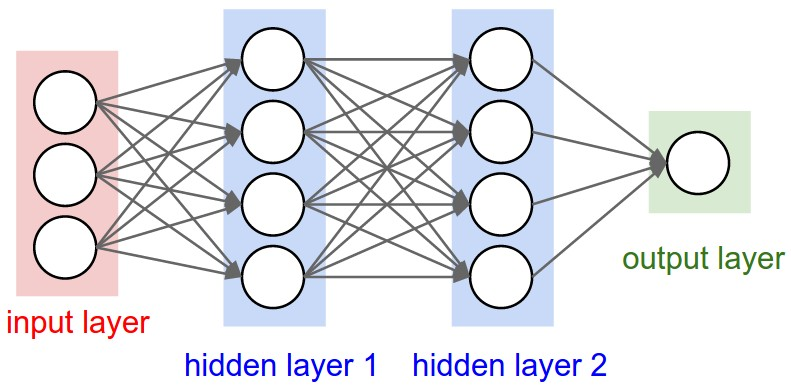
\includegraphics[width=0.5\textwidth]{neural_net}
\caption[Structure of a simple neural network.]{Structure of a simple neural network.\cite{cs231n}}
\label{fig:nn1}
\end{figure}

Let $w^l_{i,j}$ be the weight of connection from $i$-th neuron in $(l - 1)$-th layer to $j$-th neuron in $l$-th layer. Let $b_j^l$ be the bias of $j$-th neuron in $l$-th layer, $\sigma$ some activation function and $N^{(l)}$ number of neurons in layer $l$. Then the activation (output) $a_j^l$ for the $j$-th neuron in $l$-th layer is
\begin{equation}
    \label{e:activation}
    a^l_j = \sigma \left( \sum_{i=1}^{N^{(l-1)}} (w_{i,j}^l a^{l-1}_i) + b_j^l \right).
\end{equation}

We can write this more succinctly with the usage of matrices and vectors. Let $W^l$ be a weight matrix for layer $l$ which has $w^l_{i,j}$ from \autoref{e:activation} in $j$-th row and $i$-th column. Similarly let $b^l = (b_1^l, \dots{}, b_{N^{(l)}}^l)$ be a bias vector. Then we can compute an activation vector $a^l$ whose components are activations $a_j^l$ with
\begin{equation}
    \label{e:layerActivation}
    a^l = \sigma\left( W^la^{l-1} + b^l \right)
\end{equation}

Each layer produces a nonlinear transformation of outputs from previous layers. \cite{hornik} proved that standard multilayer feedforward networks with as few as one hidden layer are capable of approximating any Borel measurable function from one finite-dimensional space to another to any desired degree of accuracy. In this sense, multilayer feedforward networks are universal approximators. However, finding parameters for such networks is rather difficult.

\cite{bengio2007scaling} argues that shallow architectures can be very inefficient in terms of the required number of computational elements and examples. Furthermore, they argue that deep architectures have the potential to generalize in a way that is crucial to make progress on the kind of complex tasks required for artificial intelligence. This corresponds well with empiric observations. Commonly used \glspl{nn} have tens of layers and millions of parameters \cite{mobilenets, osnet, yolo}.

\subsection{Learning}

The goal of learning is to find the parameters $\theta = (W,b)$ (from \autoref{e:layerActivation}) that minimize the selected loss function $L(\theta)$.  Common loss functions are categorical cross-entropy for multi-class classification and \gls{mse} for regression.

Let $\theta$ be learned parameters, $Y$ the vector of target labels, also called \textit{ground truth}, and $\hat{Y}$ vector of predicted values from \gls{nn} based on $\theta$ and $N$ input vectors. Let $||.||$ be L2 norm. Then \gls{mse} is defined as:

\begin{equation}
    \label{e:mse}
    L(\theta) = \frac{1}{N} \left|\left|Y - \hat{Y}\right|\right|.
\end{equation}

With the use of a suitable cost function such as \gls{mse} and differentiable activation functions the whole \gls{nn} is differentiable and can be trained using \textit{backpropagation}. 

Backpropagation is an iterative algorithm, where we compute the gradient of the cost function with respect to the weight and then update the weights with a step proportional to the negative of the gradient. The algorithm is explained in more detail, for example in \cite{werbos1990backpropagation}.


\section{Convolutional Neural Networks}\label{s:cnns}

This section introduces \glspl{cnn}, which are a specialized kind of \gls{nn} for processing data with a known grid-like structure, for example, time-series data or images. Convolutional networks have been very successful in practical applications. The information in this section is mainly based on \cite{Goodfellow-et-al-2016} and \cite{cs231n}.

\Gls{cnn} is a \gls{nn} that uses \textit{convolution} instead of general matrix multiplication in at least one of its layers.  Convolution is a mathematical operation defined for functions $f$ and $g$ as
$$
(f * g)(t) = \int_{-\infty}^\infty f(x)\, g(t - x)\, dx
$$
in continuous and
$$
(f * g)(t) = \sum_{a=-\infty}^\infty f(a)\, g(t - a)
$$
in the discrete case. The first argument $f$ is called \textit{input} and the second argument $g$ is called \textit{kernel} of the convolution. The output is sometimes referred to as the \textit{feature map}. Convolution can be generalized to multiple dimensions.

In machine learning applications, the input is usually a \textit{tensor} (multidimensional array) of data, and the kernel is usually a tensor of learned parameters. In practice, both input and kernel are considered zero everywhere but in the finite set of points where we store their values. This allows the implementation of the infinite summation as a summation over a finite number of elements.

In traditional neural networks, the neurons in each layer are connected to all neurons from the previous layer. This large number of connections leads to a large number of parameters that need to be learned. \Glspl{cnn} leverage the structure of input data to reduce the number of parameters. If we assume that the input consists of images, we can reasonably constrain the neural network architecture.

The layers of \glspl{cnn} are arranged in three dimensions: width, height, and depth (which refers to the third dimension of an activation volume). The input layer holds the image, so its width and height will be the dimensions of the image, and the depth would be three for color images (representing the three \gls{rgb} channels).

\begin{figure}[ht]
\centering
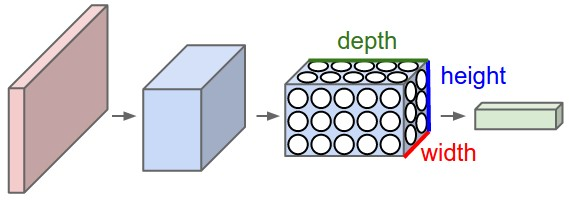
\includegraphics[width=0.5\textwidth]{cnn_3d}
\caption[\acrshort{cnn} layer transformation of 3D input volume to 3D output volume.]{\Gls{cnn} layer transformation of 3D input volume to 3D output volume.\cite{cs231n}}
\label{fig:cnn_transform}
\end{figure}

Three main types of layers are used to build \glspl{cnn}: \textit{convolutional layer}, \textit{pooling layer} and \textit{fully-connected layer}. Fully-connected layers were already introduced in section \ref{s:feed-forward}.

\subsection{Convolutional Layer}

A convolutional layer is the core building block of \gls{cnn}. Each layer consists of a set of learnable \textit{filters}. Every filter is spatially small and has the depth of the input volume. Each filter is convolved across the input volume's width and height to produce a two-dimensional activation map. Intuitively, the network will learn filters that activate when they see some feature. The idea is that early layers learn to recognize simple features like an edge, and later layers will learn to recognize more complicated patterns based on these features. The output of the whole convolutional layer is the output of each filter in given layers stacked along the depth dimension - this produces the output volume. 

Every entry in the 3D output volume can be interpreted as an output of a neuron looking at only a small region in the input and sharing parameters with all the neurons that apply the same filter. This property is called \textit{local connectivity}.

The spatial extent of this connectivity is determined by a hyperparameter called \textit{filter size}. The filter size only affects the spatial dimensions (width and height). The connectivity along the depth axis is always equal to the depth of the input volume.

Convolutional layers use a schema called \textit{parameter sharing} to reduce the number of parameters greatly. This reduction is based on the assumption that if one feature is useful to compute at some spacial position $(x,y)$, it should also be useful to compute at different positions. We can then constrain the neurons in each depth slice to use the same weights and bias. It is common to refer to this shared set of weights as a \textit{filter} (or a \textit{kernel}).

\subsection{Pooling Layer}

Pooling layers perform non-linear downsampling of the input. They do this by combining multiple values into a single value that they pass to the next layer. Most common approach is \textit{max pooling}. Max pooling takes the maximum value from its input.

It is common to periodically insert a pooling layer between convolutional layers in a \gls{cnn} architecture. The layer's function is to reduce the number of parameters, which reduces the number of computations needed and helps control overfitting.

\subsection{Transfer Learning}

\textit{Transfer learning} is a standard process, where we take a pre-trained model for a similar task and use it as initialization or a feature extractor for the target task. The use of pre-trained models dramatically reduces the computational power needed and the need for an extensive dataset.

The use of an existing \gls{cnn} as a feature extractor is simple, as only the last fully-connected layer needs to be removed or replaced.

\section{Kalman Filter}\label{s:kalman}

This section introduces \textit{Kalman filter}, which is an integral part of tracking algorithms used in this work. The information in this section is mainly based on \cite{labbe2014}.

Kalman filter is a mathematical model to gain (relatively) precise information about a system based on imprecise measurements and information about the system. Kalman filters are fairly general and have usages in estimation, data smoothing, and control applications. We will focus mainly on its usage in tracking applications.

\subsection{Introduction to g-h Filters}

Any real measurement is inaccurate. The output of any sensor does not give us perfect information about the observed system but depends on the sensor's quality. To deal with this, we can use an algorithm called \textit{g-h filter} (also called alpha-beta filter).

The first idea of the g-h filter is that the system's behavior should influence how we interpret the measurements. Imagine we are weighting a rock and getting slightly different results each time. We would probably attribute these differences to noise in the measurement. On the other hand, if we were getting changing position from a car GPS, we might conclude that the car is moving.

Assume we have some predictions for the target variable.  If we only form estimates from the measurements, then the prediction will not affect the result. If we only form estimates from the prediction, then the measurements will be ignored. This leads to the second idea that we need to take some combination of the prediction and measurement. We will call the difference between the measurement and prediction the \textit{residual}. 

In general, we cannot expect to know the rate of change of the target variable, and it also may change over time. These ideas lead to an iterative two-step process. First, we \textit{predict} the target variable and its rate of change. Next, we \textit{update} the target variable and its rate of change based on the prediction and new measurement.

This algorithm is very general. Kalman filter is then one approach on how to do these steps.

\subsection{Kalman Filter Algorithm}

Like any g-h filter, the Kalman filter makes a prediction, reads a measurement, and then forms a new estimate between the two.

The Kalman filter is using normal distributions for the representation of measurements and predictions. The normal distribution is well studied and has many interesting properties. Using normals allows us to store information about whole probability distribution as just two numbers - mean $\mu$ and variance $\sigma^2$.

Sum of two normal distributions $N(\mu_1, \sigma^2_1), N(\mu_2, \sigma^2_2)$ is a normal distribution $N(\mu_1 + \mu_2, \sigma^2_1 + \sigma^2_2)$. The product of two normal distributions is proportional to a normal distribution, meaning we can scale it to a normal distribution. These two properties mean we can sum and multiply normal distributions, and the result will still be a normal distribution (assuming we are normalizing after multiplication). 

\subsubsection*{Predict}

The general formula for the predicting the next state mean is
\begin{equation}\label{e:predict_mean}
    \overline{x} = Fx + Bu.
\end{equation}
$x$ denotes the state mean. $F$ is the \textit{state transition function}. $B$ and $u$ let us model control inputs to the system and can be removed if we do not have any control over it.

State covariance $\overline{P}$ is predicted with
\begin{equation}\label{e:predict_covar}
    \overline{P} = FPF^T + Q,
\end{equation}
where $P$ is the previosu state covariance, $F$ is the state transition function from \autoref{e:predict_mean} and $Q$ is the process covariance.

\subsubsection*{Update}

The update step consists of applying the following equations.

\begin{align}
    y &= z - H\overline{x} \\
    K &= \overline{P}H^T(H\overline{P}H^T + R)^{-1} \\
    x &= \overline{x} + Ky \\
    P &= (I - KH)\overline{P}
\end{align}

$\overline{x}, F$ and $\overline{P}, Q$ are from equations \ref{e:predict_mean} and \ref{e:predict_covar} respectively. $H$ is the measurement function. $z$ and $R$ are the measurement mean and \textit{noise covariance}. $K$ is called \textit{Kalman gain}. $I$ is the identity matrix.

Measurement noise is the variance of the sensor we are using, while process noise is the observed system variance. The measurement function maps the true state space into the observed space. 
The Kalman gain is the relative weight given to the measurements and current state estimate. With a high gain, the filter places more weight on the most recent measurements.


\subsubsection*{Summary}

\textit{Kalman filter} is a recursive algorithm that can be used to extract useful information from noisy measurements.

In the context of tracking, the Kalman filter can be used to better approximate track's bounding boxes. The Kalman state is typically some representation of a rectangle and its speed. The measurements are usually taken from a \gls{cnn}. These measurements are noisy, and the Kalman filter smooths them to provide a more accurate and stable position. Furthermore, we can also predict the track's position in the next frame, which is used to match the track to new detections. 

The filter needs correctly designed models and functions introduced in previous sections to work correctly. There is no universal approach, and the design must be based on experience, intuition, and experimentation. One possible design is described in section \ref{s:kalman_design}.

\chapter{Related Works}\label{ch:related}

This chapter presents relevant work in the area of \gls{mot} and age and gender recognition.

\section{\glsentrylong{mot}}

% what is MOT
\glsentrylong{mot} is a longstanding goal in computer vision\cite{zhang2020fair, Bewley_2016_SORT, MOT16}, which aims to estimate trajectories for objects of interest in videos.

% Tracking-by-detection as the preferred algorithm - two-step process
Tracking-by-detection has emerged as the preferred paradigm to solve the \gls{mot} problem\cite{MOT16, Wojke2017_DeepSORT}. This paradigm simplifies the task by breaking it into two steps: detecting the objects' locations independently in each frame and then forming tracks by associating corresponding detections across time. The second step is sometimes called linking or \gls{reid}.

% CNN as detectors are the way to go
In recent years,  \gls{nn}  based  detectors  have  clearly outperformed all other methods for detection.\cite{ren2015fasterRCNN, yolo}. 

% associating tracks (ReID)
Track association has been handled by various methods. Straightforward \gls{iou}\footnote{\gls{iou} of two areas is the area of their overlap over the area of their union.} based approach has been applied\cite{bochinski2017high_IOUtracking} as well as various embeddings from \glspl{nn}\cite{Wojke2017_DeepSORT}. The association step usually first computes a cost matrix based on the motion and appearance information and then matches the tracks to minimize the total cost.

% two-step method advantages
When using the two-step method, one can develop the most suitable model for both tasks separately. Additionally, one can crop and resize the image patches based on the bounding boxes before estimating the \gls{reid} features.

% combining detection and ReID - FairMOT
Recently \cite{zhang2020fair} came up with a model that handles both the detection and \gls{reid} tasks while achieving accuracy comparable to \gls{sota} trackers.\cite{MOT16}

% end-to-end approach
An alternative approach using recurrent neural networks for data association has been explored in \cite{mot_with_rnn} and \cite{mot_with_longterm}. While providing some advantages, their work is not competitive with current \gls{sota} methods.\cite{MOT16}

\subsection{\glsentrylong{sort}}\label{s:sort}

% SORT
\Gls{sort} is a pragmatic approach to \gls{mot} with a focus on simplicity and performance introduced in \cite{Bewley_2016_SORT}, which uses Kalman Filter (introduced in section \ref{s:kalman}) to predict object location in the next frame. Cost matrix is based on \gls{iou}  of Kalman predictions and detections in the new frame. Finally, Hungarian algorithm\cite{kuhn1955hungarian} is adopted to make a minimum cost matching based on the \gls{iou}.

% SORT limitations
The main disadvantage of the \gls{sort} algorithm is its reliance only on position and movement data. This can easily lead to identity switches of tracks when occluded either by environment or by other tracks.

% DeepSORT
\Gls{deepsort} extends the \gls{sort} with appearance information from a \gls{cnn}.

To incorporate motion information \gls{deepsort} uses Mahalanobis distance between predicted Kalman states and newly arrived measurement:

$$
d^{(1)}(i,j) = (d_j - y_i)^T S_i^{-1}(d_j - y_i),
$$
where $(y_i, S_i)$ is the projection of the $i$-th track into measurement space and $d_j$ is the $j$-th bounding box detection. The Mahalanobis distance takes state estimation uncertainty into account by measuring how many standard deviations the detection is away from the mean track location. This metric makes it possible to exclude unlikely associations by thresholding the Mahalanobis distance. The threshold is calculated as a $95\%$ confidence interval computed from the inverse $\chi^2$ distribution.

To incorporate appearance information we compute an appearance descriptor $r_j$ for each detection $d_j$ with $||r_j|| = 1$. Furthermore, we keep a history $\mathcal{R}_k$ of the last $L_k$ descriptors for each track $k$. We then measure the distance between the $i$-th track and $j$-th detection as the smallest cosine distance:
$$
d^{(2)}(i,j) = \min\{1 - r_j^T r_k^{(i)}\; |\; r_k^{(i)} \in \mathcal{R}_i\}.
$$

We can also find a suitable threshold to indicate if an association is admissible according to this metric using a training dataset.

We can combine both motion-based information from Mahalanobis distance and appearance-based information from the cosine distance using a weighted sum
$$
c_{i,j} = \lambda d^{(1)}(i,j) + (1-\lambda)d^{(2)}(i,j),
$$
where we call an association admissible if it is admissible for both thresholds described above.

The influence of each metric can be controlled through the hyperparameter $\lambda$.

\subsection{Metrics}

To evaluate and compare different methods, we need a way to measure errors. While this is very straightforward for some tasks, this is not the case for \gls{mot}. \cite{bernardin2008evaluating_Clear_mot_metrics} introduces two relatively simple and intuitive metrics that will be described in this section. Both metrics are widely used\cite{MOT16}.

The first metric is called \gls{motp} and characterizes trackers precision in estimating object positions. The second metric is \gls{mota} and expresses the tracker's ability to determine correct object configuration and keep consistent tracks.

The procedure for calculating these metrics consists of three steps each frame:
\begin{enumerate}
    \item establish the best possible correspondence between hypotheses and objects,
    \item for each correspondence compute the error in objects position estimation,
    \item accumulate following errors:
    \begin{itemize}
        \item count all objects with no hypothesis as misses (\textit{false negatives}),
        \item count all hypotheses with no real objects associated as \textit{false positives},
        \item count all occurrences where the tracking hypothesis for an object changed compared to previous frames as \textit{mismatches}.
    \end{itemize}
\end{enumerate}

\begin{figure}[ht]
    \centering
    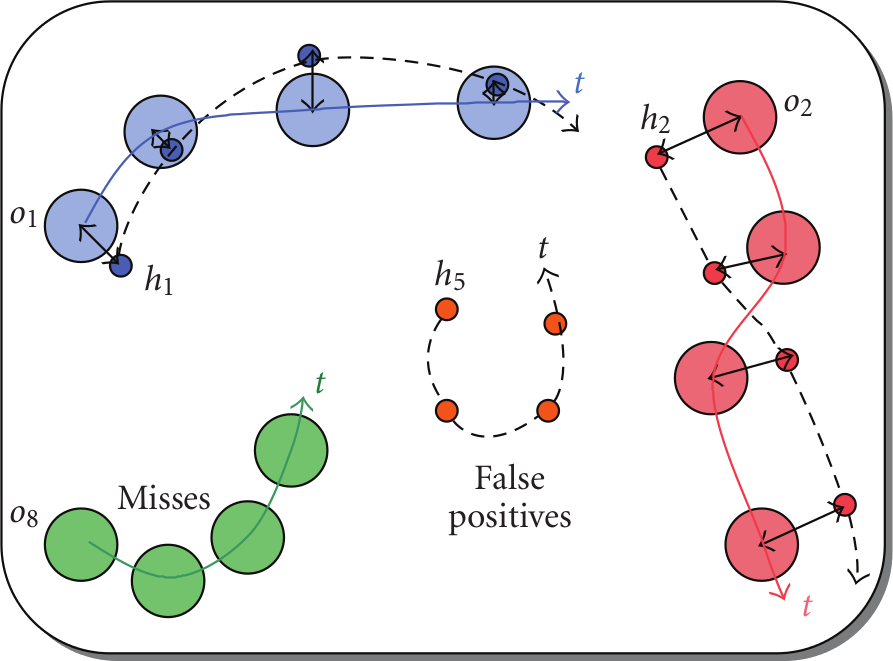
\includegraphics[width=8cm]{mot_errors}
    \caption[Illustration of various types of errors.]{Illustration of various types of errors.\cite{bernardin2008evaluating_Clear_mot_metrics}}
    \label{fig:mot_errors}
\end{figure}

Let $c_t$ be the number of matches for time $t$. For each match, let $d_t^i$ be the distance between the object and the hypothesis. The \gls{motp} is then defined as:

$$
\text{MOTP} = \frac{ \sum_{i,t}d_t^i }{ \sum_t c_t }.
$$

Let $m_t$ be the number of misses, $\mathit{fp}_t$ the number of false positives, $\mathit{mme}_t$ the number of mismatches and $g_t$ total number of objects in time $t$. The \gls{mota} is then defined as:

$$
\text{MOTA} = 1 - \frac{ \sum_t(m_t + \mathit{fp}_t + \mathit{mme}_t) }{ \sum_t g_t  }.
$$

The \gls{mota} can be seen as computed from three ratios - miss ratio, false positives ratio, and mismatch ratio.

For more discussion and implementation details see \cite{bernardin2008evaluating_Clear_mot_metrics}.

\section{Person Re-identification}\label{s:reid}

Person \gls{reid} is a fundamental task for people \gls{mot}. One person's appearance can change significantly in different frames, for example, by changing pose, turning around, or taking off a backpack. On the other hand, people often wear similar clothes and may look very similar, especially when viewed from a distance. These variations make the task challenging.

\cite{osnet} presents \textit{OSNet}, a \gls{cnn} architecture for tackling the \gls{reid} task. While \glspl{cnn} have been used before (for example in \cite{Wojke2017_DeepSORT}) to learn discriminative features for \gls{reid}, \textit{OSnet} presents a novel approach.

Key concept in \textit{OSnet} is focus on \textit{omni-scale} feature learning and its effective implementation. Authors argue that using even features at multiple scales (for example, local and global features) is not sufficient and features of all scales are crucial for the \gls{reid} task.

The result is a lightweight \gls{reid} network that achieves \gls{sota} results on multiple datasets outperforming even much bigger models.\cite{osnet}

\chapter{Analysis}\label{ch:analysis}


The main goal of this work is to create a pipeline for processing video data, with the goal of consistently tracking people in front of a retail shop. Additionally, we want to extract age and gender information for found tracks.

This chapter discusses this objective in more detail to allow us to design and evaluate a solution. To keep the scope manageable while keeping the application usable in a real-world environment, we have to make some assumptions about the observed environment (inputs). These assumptions should be noted so the limitations of the system are clear.

%%%%%%%%%%%%%%%%%%%%%%%%%%%%%%%%%%%%%%%%%%%%%%%%%%%%%%%%%%%%%%%%%%%%%%%%%%%%%%%%%%%%
\section{Target Environment}

The target environment is an area in front of a retail shop. This area can be outdoors or indoors, for example, inside a shopping mall.

We assume a single stationary camera recording this environment. Each environment is different, so the setup must be adjusted individually to provide the best possible video quality. A specific setup used for data acquisition for this work will be described in a later chapter.

Since only one camera can be used, it must be carefully positioned to capture the whole area of interest with reasonable quality. The area is also expected to be well lit, meaning the system is not expected to work, for example, at night, unless suitable artificial lighting is provided.

On the other hand, imperfect conditions are expected in real environments. The system should deal with minor lighting changes and reflections caused by the environment and various distortions caused by the camera. For example, reflections from the shop windows are expected. The camera system should be selected and installed in a way to minimize these problems.

%%%%%%%%%%%%%%%%%%%%%%%%%%%%%%%%%%%%%%%%%%%%%%%%%%%%%%%%%%%%%%%%%%%%%%%%%%%%%%%%%%%%
\section{Dataset}\label{s:dataset}

An appropriate dataset is required to tune and evaluate the algorithm. \cite{MOT16} presents multiple datasets from various scenes along with annotations. These datasets are commonly used for evaluation in literature. Both datasets and evaluation results are available at \url{https://motchallenge.net}. This dataset's main advantages are that it allows for direct comparison with many different tracking algorithms and provides ground truth annotations.

\begin{figure}[ht]
    \centering
    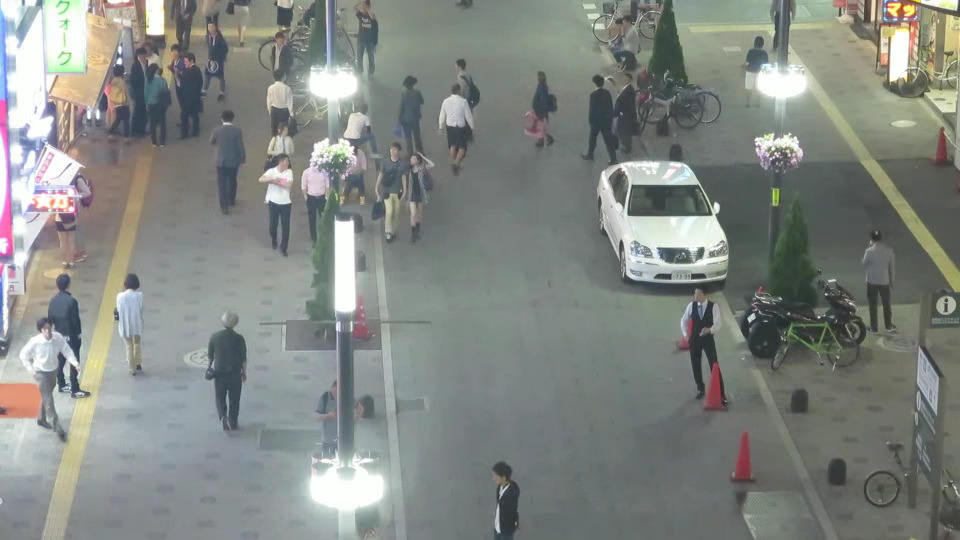
\includegraphics[height=3cm]{MOT16_sample}
    \caption{Example frame from the \cite{MOT16} dataset.}
    \label{fig:mot_sample}
\end{figure}

We have decided to create our dataset targeting the retail environment, as we have not found any usable data from the specified environment. Such a dataset will be more representative and allow for more accurate evaluation. Further, it can be used to optimize and fine-tune the system for the target environment. 

Dataset collection was done in cooperation with store owners, where the designed system might be used in the future. This cooperation allowed us to collect the dataset according to the system's assumed use. Collecting the dataset in the retail environment has shown some complications the system might face in actual usage and helped significantly with problem analysis from a practical standpoint.

The dataset collection process was done across two locations. The first location was used for selecting a camera, finding suitable camera placement, and initial experiments. The dataset itself was collected at the second location.

\subsection{Camera Selection}

This section describes the first part of the dataset collection process, where short videos were recorded with multiple cameras in different positions at the first location.

Cameras were placed in a shop window behind glass with the view facing the street. Evaluation criteria were image quality, camera view (does the camera see the full \gls{roi}), and camera noticeability. Camera noticeability is meant as a criterium of how much the camera is visible to a passerby, as a noticeable camera might discourage potential customers from browsing the shop window.

Three possible camera placement configurations were considered:
\begin{enumerate}
    \item at the edge of the shop window, near the glass, at approximately 150 cm from the ground,
    \item at the center of the shop window, near the glass, at approximately 150 cm from the ground,
    \item at the edge of the window in the corner, at approximately 220 cm from the ground, positioned at an angle.
\end{enumerate}

The first option did not present a sufficient view of the \gls{roi} and was rejected. The second option provided good image quality while being more noticeable. The third option proved to be very unobtrusive with a good view. However, the image quality seemed subjectively slightly lower, mainly thanks to reflections on the glass window.

Recordings from the second and third configurations were further evaluated using a simple initial version of the tracking algorithm. This early evaluation confirmed the third configuration as suitable and hinted at the task as being reasonably solvable. 

Based on the initial testing, the AXIS FA1105 surveillance camera\cite{axis_fa1105} was selected for the following recordings. This camera is highly discreet, provides sufficient video quality with resolution 1920x1080 (1080p), and has a wide $111\degree$ horizontal field of view.

\subsection{Dataset Acquisition}\label{s:dataset_acquisition}

Before starting the dataset collection itself, we needed to find a suitable camera configuration for the second location, which proved to be more challenging than expected. The camera was placed at a shop inside a shopping mall. The main difficulties were caused by camera obtrusiveness and appearance, lighting conditions, and reflections.

The camera appearance issue was solved by 3D printing a custom camera holder, which allowed for a more discrete and pleasant camera look. One of the main lighting problems was direct lighting from the shopping mall ceiling, which was handled by adding a black cover on top of the camera to shield it from this lighting. The camera is shown in figure \ref{fig:camera}.

\begin{figure}[ht]
    \centering
    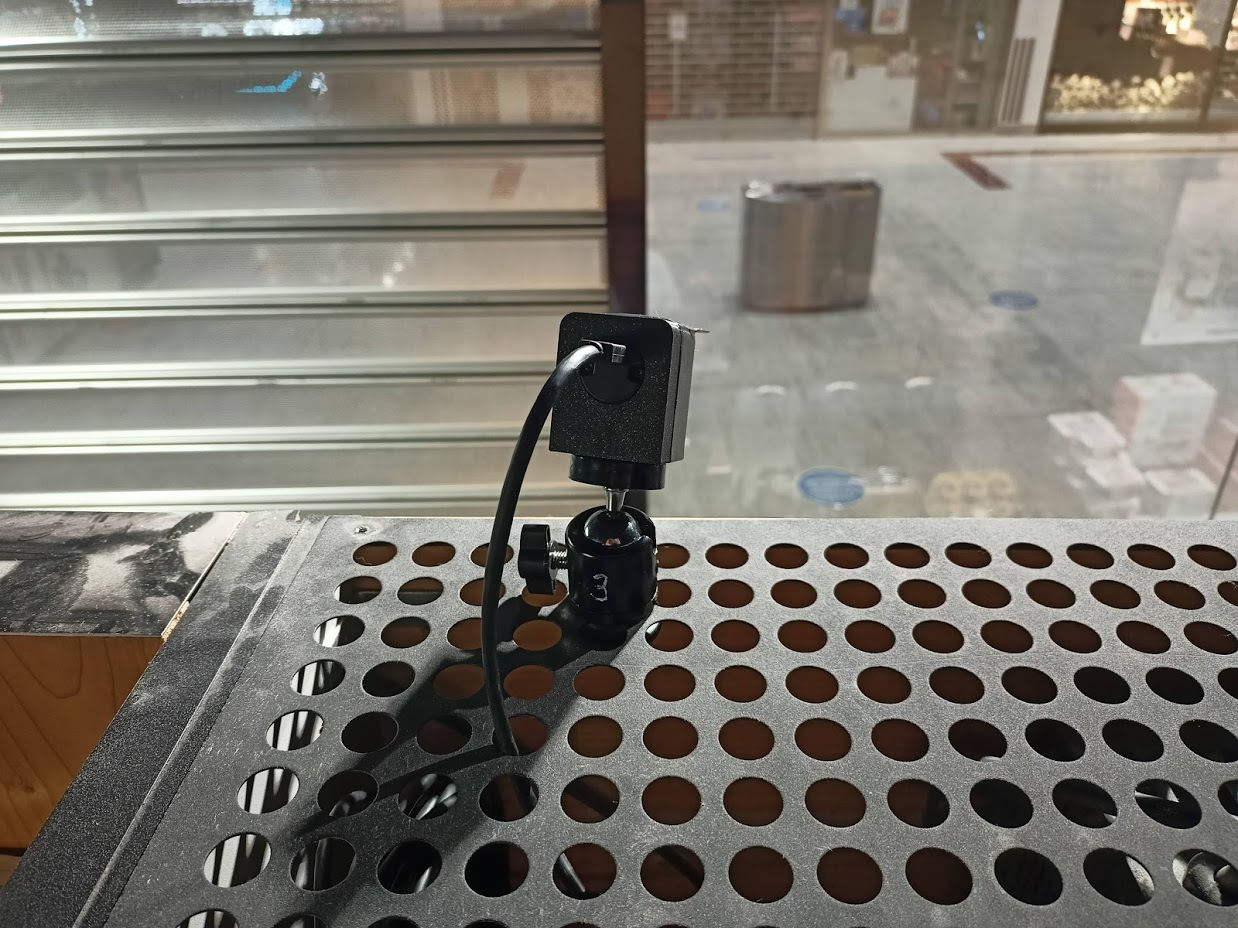
\includegraphics[width=5cm]{camera_back}
    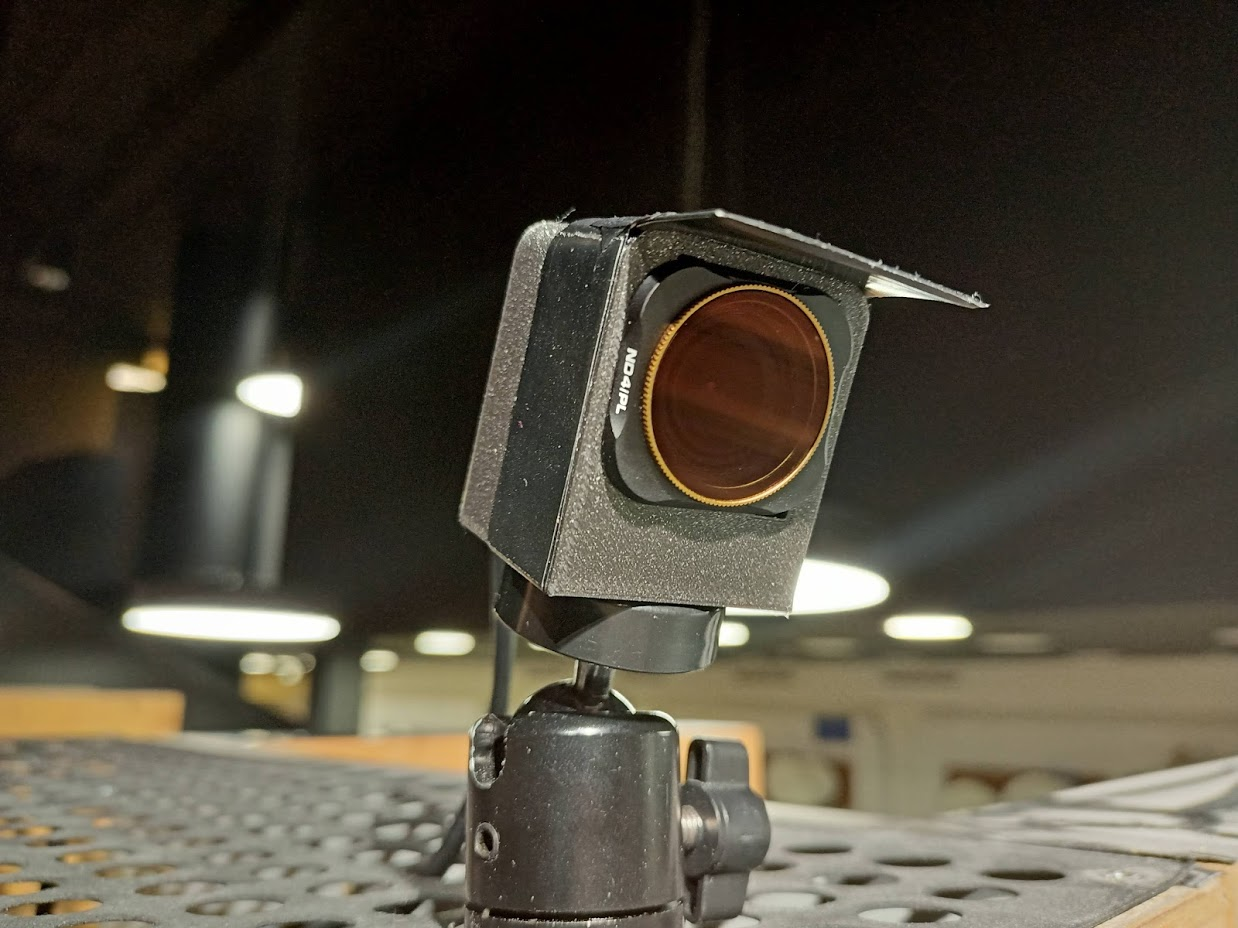
\includegraphics[width=5cm]{camera_front}
    \caption{Camera used for dataset acquisition.}
    \label{fig:camera}
\end{figure}

Another significant problem was reflections on the shops' glass windows. A polarization filter was added to the camera to minimize these reflections. While this improved the image quality, reflections remain a problem. The effect can be seen in figure \ref{fig:polarizer}.

\begin{figure}[ht]
    \centering
    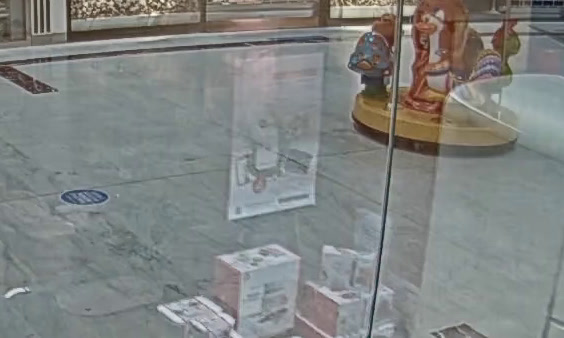
\includegraphics[width=5cm]{polarizer_bad}
    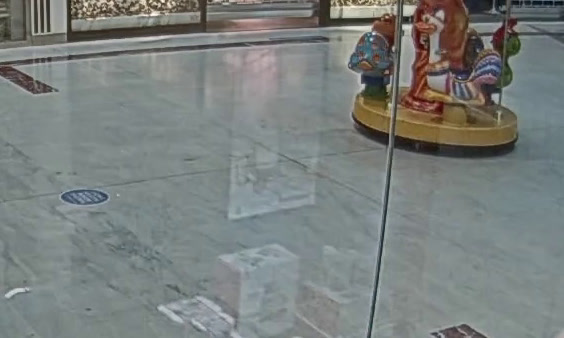
\includegraphics[width=5cm]{polarizer_good}
    \caption[Image taken without a polarizer filter and with polarizer filter.]{Image taken without a polarizer filter (left) and with polarizer filter (right).}
    \label{fig:polarizer}
\end{figure}

The camera remained in the location long-term, however usable dataset size is limited by the time needed to annotate the data. Multiple video sequences were hand-selected and annotated using CVAT software\cite{cvat}. The total dataset size is 2600 annotated frames. A sample dataset frame can been seen in figure \ref{fig:dataset_sample}.

\begin{figure}[ht]
    \centering
    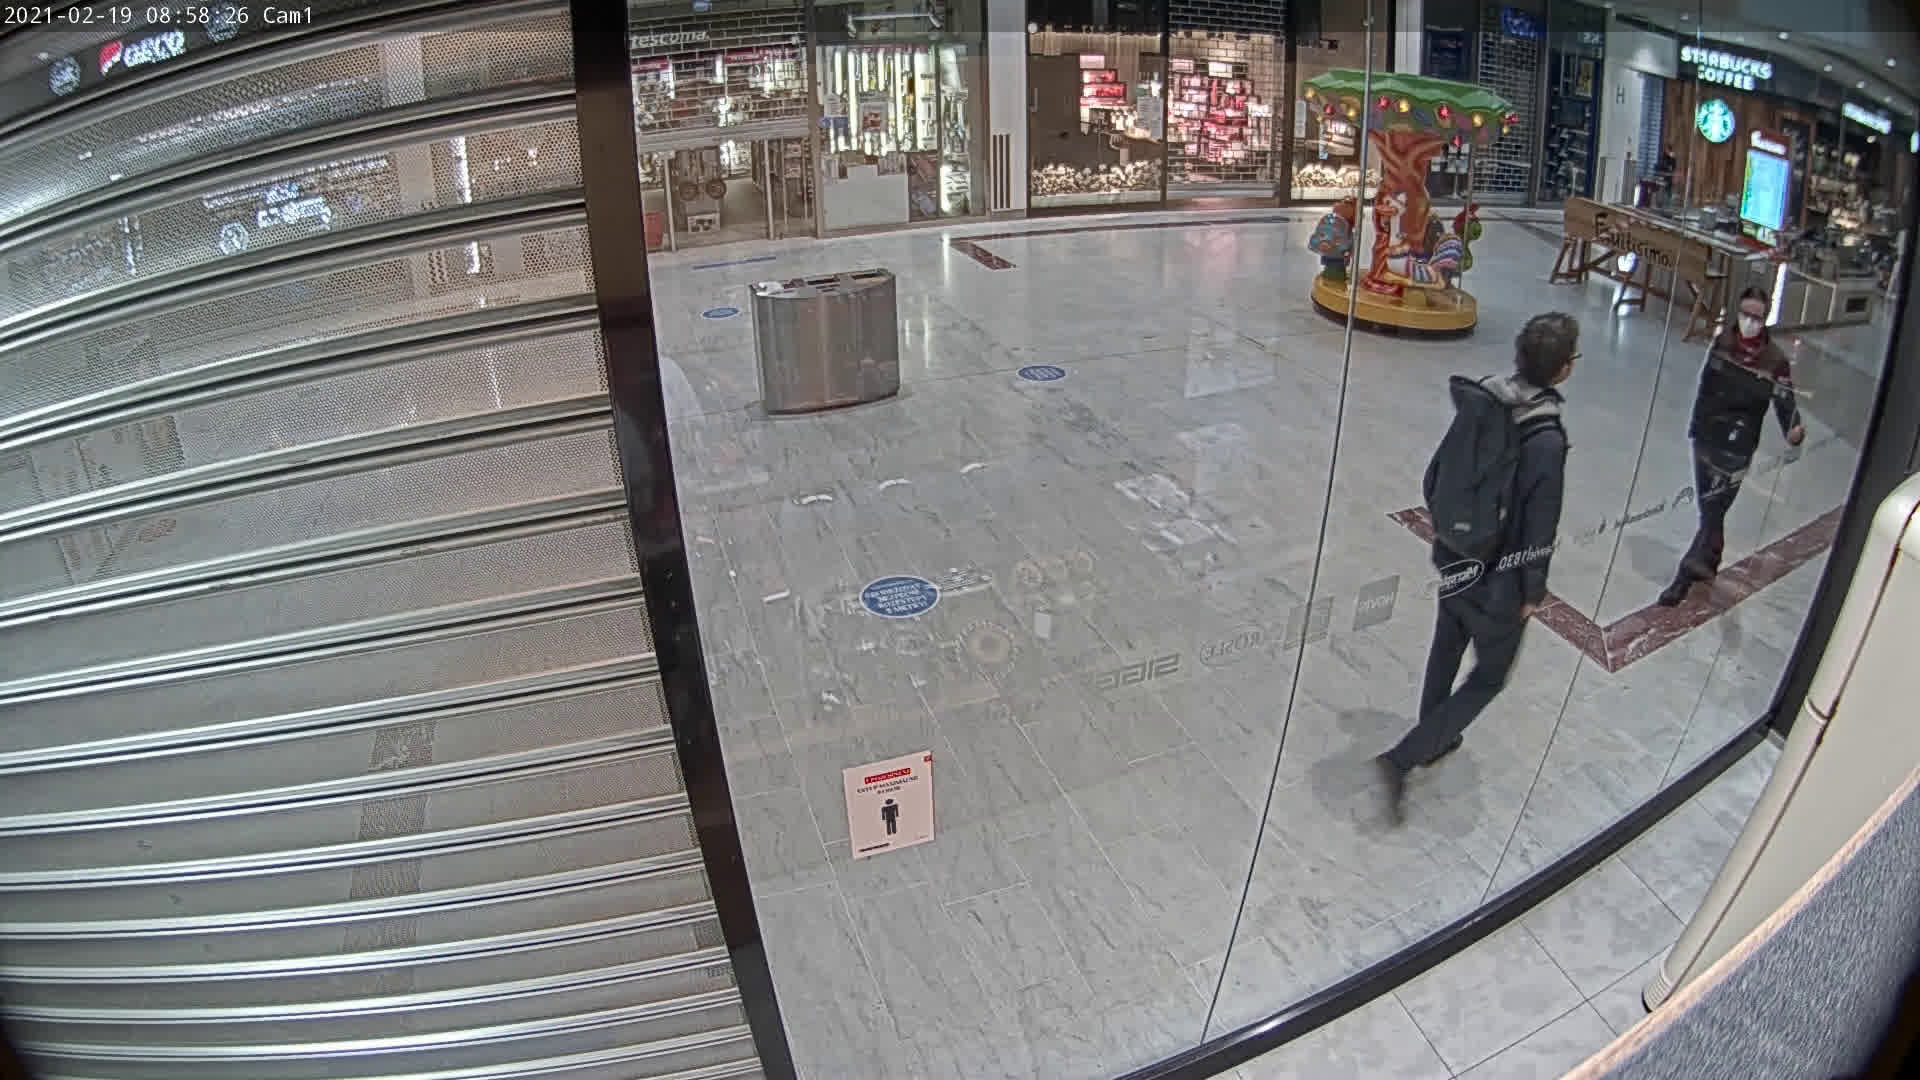
\includegraphics[width=8cm]{dataset_sample}
    \caption{Sample frame from collected dataset.}
    \label{fig:dataset_sample}
\end{figure}

\subsection{Region of Interest}

The goal of our work is to observe a region in front of a shop. It can be expected that the camera captures a larger area, as is the case in our collected dataset. The tracks need to be filtered based on their position to select only the tracks in the target area to provide relevant statistics.

The \gls{roi} is also relevant for the experimental evaluation. Evaluating tracks only in \gls{roi} makes the evaluation more relevant to the actual goal. Tracking people far away from the shop (and the camera) is not our goal and may not be reasonably achievable. Tracks in a significant distance are small, their image resolution is low, and occlusions and bounding box overlaps make this even more difficult. What is considered relevant needs to be considered for each camera setup individually.

To filter the relevant tracks, we need to specify a function to tell if a given track lies inside the \gls{roi}. The target area could be intuitively specified as a polygon. More general shapes could allow more flexibility but increase the complexity of operations such as intersection. Once we have the target area specified as some geometric shape, we can find if a track is inside based on bounding box intersection. Simple intersection could also be expanded to consider, for example, only tracks above some intersection over minimum threshold. Another possible approach is to convert each track to a single point (such as its bounding box center) and then find if the given point lies in the \gls{roi}.

The methodology used for evaluation is described in chapter \ref{ch:experiments}.

\subsection{Age and Gender Information}\label{s:dataset_age_and_gender}

The original goal for the dataset was to include age and gender information. This was an additional reason for collecting our dataset, as we do not know any \gls{mot} dataset that includes the biometric information. The current Covid-19 epidemic complicates the task significantly, as (nearly) all people wear face masks.

Initial experiments on collected data confirmed that extracting biometric information on images with face masks is challenging and currently available models and datasets are not sufficient for this task. Furthermore, we did not find any relevant datasets and little relevant work, which is probably caused by how unexpected and novel the current pandemic situation is.

Dealing with face masks properly is out of scope for this work. We consider the mask situation temporary, so it is not essential for future use of the application.

Based on the current difficult situation, we have made the following decisions. We do not include the age and gender information in our collected dataset. We include the age and gender classification in our pipeline; it is prepared for use once the situation with face masks changes. We evaluate the age and gender models mainly from the performance standpoint.

%%%%%%%%%%%%%%%%%%%%%%%%%%%%%%%%%%%%%%%%%%%%%%%%%%%%%%%%%%%%%%%%%%%%%%%%%%%%%%%%%%%%
\section{Age and Gender Classification}

% we want to extract age and gender -> use CNNs
One of the goals of this thesis is to extract age and gender information for tracked people. Multiple works dealing with this task exist, using various \gls{cnn} architectures\cite{levi2015age, yang2018ssr, karkkainenfairface}.

% you can use the same architecture for both tasks
The same network architecture can typically be used for both age and gender as in \cite{levi2015age}, except the last layer, which has to match the target number of classes.

% output
The expected output for gender is either male or female. For age information, the output format is less straightforward.

% output - classification vs regression
While age estimation has been formulated as a regression problem, for example, in \cite{yang2018ssr}\footnote{Even \cite{yang2018ssr} is based on classification that is turned into regression using expected values.}, it is more common to formulate it as a classification problem, where the categories are various age ranges\cite{levi2015age, karkkainenfairface}.

% output - use classification
Formulating the age prediction as a classification task into some age ranges simplifies the task (as we do not try to predict the exact age) and arguably does not reduce the information usefulness noticeably. Marketing strategies and behavior prediction will probably be different for various age groups, such as children, adults, and the elderly, but differ less inside these groups.

\subsection{Classification Input}

% input - body vs face
The required information can be extracted either from a whole-body image or from a face image. Using a whole-body image would be very beneficial since this information is always available, and no association step is needed. \cite{pavlakos2019expressiveBody} explores gender classification based on body pose estimation, which is in turn based on image information. We experimented briefly with this approach and found both performance and accuracy to be insufficient.

% input - face
A more typical approach is to use face information\cite{levi2015age, yang2018ssr, karkkainenfairface}, which has its own downsides. The face may not always be visible, and we need to associate faces to appropriate tracks.

% input - video (not single image)
In contrast to classification on a single image, our input is a sequence of frames. We need for a given face to be visible on at least one frame to make predictions. While this provides no guarantees, it makes the chance of a successful face detection more likely. If we have multiple predictions for a single track, we need to put them together using some statistical function such as mean or median.

\subsection{Face Alignment}

Both literature\cite{karkkainenfairface} and our experiments suggest that the classification task is heavily influenced by face alignment. We found that many detected faces are practically unusable for prediction because of alignment and general image quality issues.

As a potential improvement, we experiment with filtering faces based on face alignment. The goal is to accept predictions that are based only on face images with reasonable quality and alignment.

%%%%%%%%%%%%%%%%%%%%%%%%%%%%%%%%%%%%%%%%%%%%%%%%%%%%%%%%%%%%%%%%%%%%%%%%%%%%%%%%%%%%
\section{Hardware and Performance}

Most tracking and age and gender classification methods use \glspl{nn} as described in previous chapters. One of the limiting factors of \glspl{nn} is the computing power they require\cite{MOT16, yolo}.  Advances both in theoretical understanding and hardware have allowed for \glspl{nn} to be used in an increasing number of devices such as mobile phones\cite{mobilenets} and even browsers\cite{tfjs}.

However, video processing is still a very data-intensive task. Processing live feed requires processing multiple images each second. One of the system's primary goals should be to focus on speed to allow live camera feed processing.

Furthermore, using a dedicated (edge) device that would process the video stream at the camera's location would significantly improve the system's scalability and ease of use.

For these reasons, \gls{Jetson}\cite{jetson} was chosen as a testing device, which will be used to process the video stream and run the tracking algorithm in our experiments. This device is very compact and specialized for both video processing and \glspl{nn} inference, making it suitable for use in the retail environment. Running all experiments on single hardware assures that the results are comparable when looking at processing time. Running on a suitable device for the production environment also makes the results more directly relevant and usable.

\subsection{Optimization}

In recent years, there has been growing interest in building \gls{ai} models with the focus not only on quality but also on performance (computation power required)\cite{yukai_yang_2020_4294717_fastmot,tracktor_2019_ICCV,yolo}. Performance can often be significantly increased when using a smaller model\footnote{By smaller, we mean model with less learnable parameters. For \glspl{nn} the critical factor is typically depth; however, the overall architecture is also important.} without significant quality loss\cite{yang2018ssr}.

Another important topic is optimization of existing models. The task of reducing \gls{nn} size by removing parameters is called \textit{pruning}\cite{blalock2020stateOfPruning}.

A common pruning strategy\cite{blalock2020stateOfPruning} is to first train the target \gls{nn} to convergence. After which parameters or structural elements are issued a score. The network is then pruned based on these scores. Pruning typically reduces\footnote{Pruning can also increase the accuracy in some cases\cite{Molchanov_2019_CVPR_improtanceEstimationForPruning}.} the accuracy of the network, so the network can then be trained further (this is called \textit{fine-tuning}).

NVIDIA TensorRT\cite{vanholder2016efficientTensorRT} is a framework for \gls{nn} optimization and efficient inference. This software is closed-source, and the precise optimization algorithm is not disclosed. We will evaluate it experimentally in chapter \ref{ch:experiments}.

\chapter{Design}\label{ch:design}

This chapter presents our proposed tracking algorithm. Our solution is based on the \gls{deepsort}\cite{Wojke2017_DeepSORT} algorithm, introduced in section \ref{s:sort}. Implementation, especially with respect to efficient use of hardware, has been inspired by \cite{yukai_yang_2020_4294717_fastmot}. 

We use the following notation. \textit{Track} is each unique object of interest (in our case person). Track's \textit{age} is the number of frames it has not been associated with any detection. We will say a track is \textit{active} if its age is below some threshold.  We say track is \textit{confirmed} if it has been associated with a detection at least $n$ times. Track is considered \textit{lost} if it moves out of the frame or is not matched with a detection for $m$ frames.

The algorithm consists of the following high-level steps which are run for each input frame.

% ~ MOT.step
\begin{enumerate}
    \item detect people and faces % detector
    \item extract visual features from detections % feature extractor 
    \item apply Kalman filter % tracker.apply_kalman
    \begin{enumerate}
        \item run prediction for each existing track
        \item mark/remove tracks that move out of frame
    \end{enumerate}
    \item associate existing tracks with detections and update tracks % tracker.update
    \begin{enumerate}
        \item associate \textit{confirmed} tracks based on Mahalanobis distance and visual features 
        \item associate remaining \textit{confirmed} and \textit{active} tracks based on \gls{iou}
        \item associate \textit{unconfirmed} tracks based on \gls{iou}
        \item associate (\gls{reid}) \textit{lost} tracks based on visual features
        \item update tracks % update matched, update not matched (delete/mark_missed/mark_lost)
        \item register new tracks
    \end{enumerate}
    \item extract biometric information from faces
    \item associate faces to tracks
\end{enumerate}


\begin{figure}[htb]
    \newcommand{\mysize}{0.4\textwidth}
     \centering
     \begin{subfigure}[b]{\mysize}
         \centering
         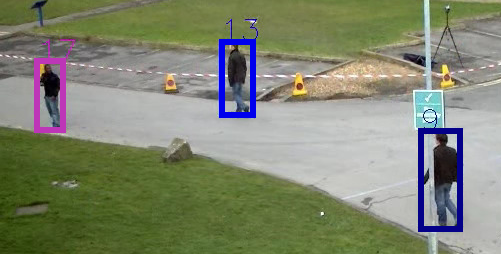
\includegraphics[width=\textwidth]{algo/tracks_at_t0.png}
         \caption{Tracks at time $t$.}
         \label{fig:tracks_at_t0}
     \end{subfigure}
     \hfill
     \begin{subfigure}[b]{\mysize}
         \centering
         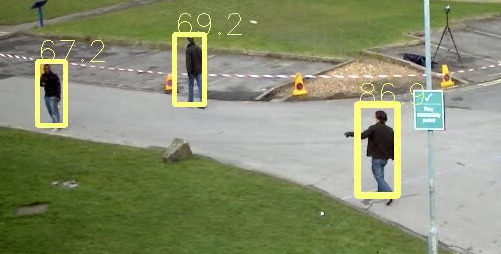
\includegraphics[width=\textwidth]{algo/detections_at_t1.png}
         \caption{Detections at $t + 1$.}
         \label{fig:detections_at_t1}
     \end{subfigure}
     \hfill
     \begin{subfigure}[b]{\mysize}
         \centering
         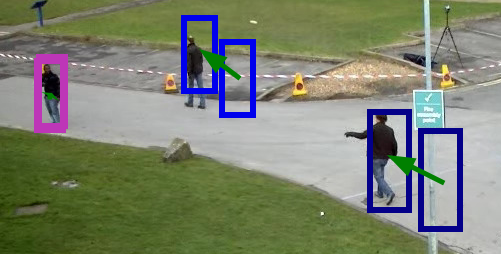
\includegraphics[width=\textwidth]{algo/kalman_predictions_for_t1.png}
         \caption{Kalman predictions for $t + 1$.}
         \label{fig:kalman_predictions_for_t1}
     \end{subfigure}
     \hfill
     \begin{subfigure}[b]{\mysize}
         \centering
         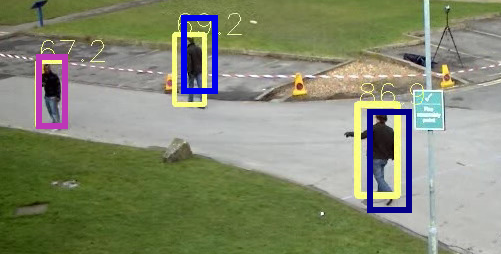
\includegraphics[width=\textwidth]{algo/iou_at_t1.png}
         \caption{Matching is based on \gls{iou} and visual features.}
         \label{fig:matching_at_t1}
     \end{subfigure}
     
    \caption[Visualisation of the main tracking steps.]{Visualisation of the main tracking steps. Images from \cite{MOT16}, modified.}
    \label{fig:simplified_algorithm}
\end{figure}


\section{Detection and Feature Extraction}

\Glspl{cnn}, which were introduced in section \ref{s:cnns}, provide \gls{sota} results for the tasks of detection, feature extraction and age and gender classification. Many \gls{cnn} architectures exist, and the choice of the appropriate one is not obvious. The training dataset selection is also essential.

Our criteria for model selection are accuracy, speed, and, for practical reasons, availability of pre-trained models.

Since performance is a priority, the model should detect both faces and people. Furthermore, we could increase performance if the network used for detection also provided visual features, which would remove the need for a dedicated feature extractor network. \cite{zhang2020fair} proposes such a network while claiming good performance. We found their model to be too slow for real-time processing on our hardware. However, their approach seems very promising, and combining detection and feature extraction might be the best approach in the future.

Comparison of various models is presented in chapter \ref{ch:experiments}.

Based on our analysis, we selected YOLOv4\cite{bochkovskiy2020yolov4} model as the detection model. We use version pre-trained on \cite{shao2018crowdhuman} dataset, with potential fine-tuning on data from the target environment. 

For feature extraction we use \textit{OSnet} architecture from \cite{osnet}, which achieves \gls{sota} results on multiple \gls{reid} datasets and is very lightweight. For details see section \ref{s:reid}. Specifically we use the the version termed \texttt{osnet\_x0\_25} trained on the MSMT17\cite{wei2018person_msmt17} dataset. Pre-trained model is  provided by the paper authors.



\section{Kalman Filter Design}\label{s:kalman_design}

We use the Kalman filter to predict each track's position and update its position after association with a detection. General introduction to Kalman filter is presented in \ref{s:kalman}. This section describes the Kalman model used and its application in our algorithm.

\subsection{Model Design}\label{s:kalman_model_design}

We define the \textit{Kalman state} as a vector
$$
x = ( x_1, y_1, x_2, y_2, \dot{x}_1, \dot{y}_1, \dot{x}_2, \dot{y}_2 ),
$$
where the first four elements represent the coordinates of the top left and bottom right points of the track's bounding box, and the remaining elements are their respective velocities.

Each track is then represented by state means vector $x \in \mathbb{R}^8$ and covariance matrix $P \in \mathbb{R}^{8,8}$. The means vector is initialized from detection with its coordinates and zero velocity. We initialize the covariance matrix as a diagonal matrix. The specific values depend on the observed scene and quality of the detector model.

We assume a constant velocity model for the tracked objects. This assumption is common in literature \cite{Bewley_2016_SORT, Wojke2017_DeepSORT, labbe2014}. Human motion is generally not linear. However, the Kalman filter can reasonably work even when the assumption is not satisfied.

With the constant velocity model in mind, we can define \textit{state transition function} $F$ as
$$
F = \begin{bmatrix}
 1 & 0 & 0 & 0 & 1 & 0 & 0 & 0 \\
 0 & 1 & 0 & 0 & 0 & 1 & 0 & 0 \\
 0 & 0 & 1 & 0 & 0 & 0 & 1 & 0 \\
 0 & 0 & 0 & 1 & 0 & 0 & 0 & 1 \\
 0 & 0 & 0 & 0 & 1 & 0 & 0 & 0 \\
 0 & 0 & 0 & 0 & 0 & 1 & 0 & 0 \\
 0 & 0 & 0 & 0 & 0 & 0 & 1 & 0 \\
 0 & 0 & 0 & 0 & 0 & 0 & 0 & 1 \\
\end{bmatrix}.
$$

Next, we define \textit{measurement function} $H$, which is used to transition from the Kalman state space to a measurement space. In our case, this means moving from an 8-dimensional vector with position and velocity to a 4-dimensional vector with only the position. The measurement function is
$$
H = \begin{bmatrix}
 1 & 0 & 0 & 0 & 0 & 0 & 0 & 0 \\
 0 & 1 & 0 & 0 & 0 & 0 & 0 & 0 \\
 0 & 0 & 1 & 0 & 0 & 0 & 0 & 0 \\
 0 & 0 & 0 & 1 & 0 & 0 & 0 & 0 \\
\end{bmatrix}.
$$

The remaining parts to define are \textit{measurement noise} matrix $R$ and \textit{process noise} matrix $Q$. We define the measurement matrix as a diagonal matrix $R \in \mathbb{R}^{4,4}$ with $\alpha \in \mathbb{R}^+$ on the diagonal. In practice the $\alpha$ value is a hyperpameter based on the precision of the underlying detector model.

We model the process noise as a discrete white noise. Let $\beta \in \mathbb{R}^+$ be a hyperparameter, then the process noise matrix is
$$
Q = \beta \cdot \begin{bmatrix}
 0.25 & 0    & 0    & 0    & 0.5 & 0   & 0   & 0   \\
 0    & 0.25 & 0    & 0    & 0   & 0.5 & 0   & 0   \\
 0    & 0    & 0.25 & 0    & 0   & 0   & 0.5 & 0   \\
 0    & 0    & 0    & 0.25 & 0   & 0   & 0   & 0.5 \\
 0.5  & 0    & 0    & 0    & 1   & 0   & 0   & 0   \\
 0    & 0.5  & 0    & 0    & 0   & 1   & 0   & 0   \\
 0    & 0    & 0.5  & 0    & 0   & 0   & 1   & 0   \\
 0    & 0    & 0    & 0.5  & 0   & 0   & 0   & 1   \\
\end{bmatrix}.
$$

\subsection{Predict and Update}

\textit{Predict} and \textit{update} are the basic steps of the Kalman algorithm. In the prediction part, we try to predict the Kalman state for the next time step.

The update step is based on a measurement $z$. In our algorithm, the measurement is a bounding box of detection associated with the given track. Update consists of computing \textit{residual} $y$ and \textit{Kalman gain} $K$ and then updating the Kalman state. Kalman gain affects how much weight we place on the measurement when combining it with the prediction.

Let $x_t \in \mathbb{R}^8, P_t \in \mathbb{R}^{8,8}$ be the state mean and covariance of the given track at time step $t$. State mean and covariance are separate for each track and time step.

Further, let $F, H, Q, R$ be the various matrices defined in the previous section.

The \textit{predict} step is described by the following equations:
\begin{align}
    \hat{x}_{t+1} &= Fx_t , \\
    \hat{P}_{t+1} &= FPF^T + Q,
\end{align}

and the standard update step is described by:
\begin{align}
    y &= z - H\hat{x}_{t+1} ,\\
    K &= \hat{P}_{t+1} H^T (H \hat{P}_{t+1} H^T + R)^{-1} ,\\
    x_{t+1} &= \hat{x}_{t+1} + Ky ,\\
    P_{t+1} &= (I - KH)\hat{P}_{t+1} .\label{eq:P_update}
\end{align}

We replace equation \ref{eq:P_update} with the following, more numerically stable version from \cite{appliedKalman}:
$$
P_{t+1} = (I - KH)\hat{P}_{t+1}(I - KH)^T + KRK^T.
$$
 
 
% describe how we use it - we run it each frame to predict and then update to smooth detections
\subsection{Application}

We run the Kalman filter on each input frame. First, the \textit{prediction step} is run, and the predicted Kalman state is assigned as a new state to all tracks. This new state is then used for all operations in the algorithm's association step (described in the next section). If the intersection over minimum of the input frame and the track's newly computed bounding box is less than 0.5, the track is considered to have left the scene and is marked as lost.

When using the Mahalanobis distance, both mean and covariance are used for the distance calculation. However, when using \gls{iou} between detections and tracks, only the bounding box information is required. The bounding box information can be extracted easily using the measurement function\footnote{In our case, this simply means taking the first four elements of the state, but in general, the transformation could be more complex.}.

After the detections and tracks are associated, we run the \textit{update step} for each track for which detection was associated. The input measurement is the bounding box of the detection. We also check if the track left the scene same way as in the prediction step.

\section{Track Association}
Associating tracks and detections is a non-trivial task. The tracker has to differentiate between missed detections and objects leaving the scene. It has to decide wherever unmatched detection is a new track or just a false positive.

To make the tracker more robust and accommodate for various errors in underlying models, we perform the matching in multiple steps. We prioritize already established tracks and wait for multiple frames before marking the track as confirmed.

% Why are identity switches bad?
% - because they are hard to detect and fix even if we consider offline postprocessing
% - because they introduce long-term errors, whereas the false positives and false negatives are typically short-term
We find the identity switches as the most relevant and detrimental type of error, because they introduce long-term errors, whereas the false positives and false negatives are typically short-term and do not disrupt the overall trajectory. 

Identity switches can easily happen in groups of multiple people, where the algorithm cannot rely on the position information. Moreover, even relevant visual information can be difficult to obtain due to occlusion. Problematic situations may also be caused by partial or full occlusions from the environment and different visual conditions in various parts of the input frame.

% tady pak už popsat jednotlivý kroky tý asociace
\subsection{Association Steps}

% general
The main part of all association steps is forming a cost matrix for a subset of tracks and a subset of detections. The cost matrix contains the distance between given tracks and detections. Once we have this matrix, we can easily find the minimum cost matching using one of the standard algorithms in polynomial time\cite{kuhn1955hungarian, bourgeois1971extension_munkers}. We start the association with all defections\footnote{By all detections we mean all detections of appropriate class with at least given confidence.}. Detections matched in any step are not used in subsequent steps.

% association - ours vs DeepSort
The first association step is analogical to \gls{deepsort}\cite{Wojke2017_DeepSORT}, which is described in section \ref{s:sort}, with differences described further. The remaining steps are mostly inspired by \cite{yukai_yang_2020_4294717_fastmot}.

% 1st step
In the first step, we associate only \textit{confirmed} tracks. The cost matrix is computed based on Mahalanobis between tracks' states and detections' bounding boxes and feature vectors similarity. Apart from using only the confirmed tracks, another difference from the original \gls{deepsort} is how we store the visual features. The original keeps a gallery of the last $n$ features for each track and computes the distance as a minimum distance between any feature in the gallery and the bounding box feature. 

% 1st step - gallery vs "smooth feature"
Instead of this, we keep only a single feature (vector) for each track. On update, the new feature is calculated as a weighted average of the current and new feature and is normalized afterward. This approach is faster since we need to compute only a single distance for each track. An additional advantage is a potential for robustness. When using the gallery, a single incorrect measurement can take precedence over multiple valid measurements and can remain in the gallery for a long time. 

% 2nd association
In the second step, we associate the \textit{confirmed} tracks which were not associated with any detection in the first step. We also filter out tracks that are not active. The cost matrix is computed based only on \gls{iou} of tracks and detections' bounding boxes.

% 3rd association
The third step associates unconfirmed detections. The cost matrix is computed from \gls{iou} of tracks and detections' bounding boxes, as in the previous step.

% lost tracks re-id
After that, \textit{lost} tracks are associated based only on visual features. This step is similar to the first one; however, no position information is used, as we cannot meaningfully predict the position of lost tracks.

% update matched
Next, we update all matched tracks and set their age to zero. We update their Kalman filter state as described in the previous section.

% cleanup tracks
The next part is dealing with unassociated tracks. We remove those which are unconfirmed, dismissing them as a false positive. We increase the age of remaining unmatched tracks. If the track's age is above some threshold, we mark it as lost.

% register new detections
The last step is creating new tracks from the remaining detections. We initialize each track with a Kalman state as described in section \ref{s:kalman_model_design}.

\section{Age and Gender Classification}

This section describes the age and gender classification of faces and subsequent association with tracks. We introduce optional step for filtering faces based on face alignment. Additionally, we discuss how to produce a final outcome from multiple classification results.

We will be using \glspl{cnn} for the classification task. We find the architectures \textit{GoogLeNet} from \cite{szegedy2015going_googlenet} and \textit{SSRNet} from \cite{yang2018ssr} to be suitable for use in our algorithm. We chose these based on their speed and proclaimed accuracy, as we cannot properly evaluate them due to the dataset problems described in section \ref{s:dataset_age_and_gender}.

\subsection{Face Association}

To propagate the age and gender information to the tracks, we need to associate them with the faces. We calculate a center point for each face's bounding box. We then (for each face) iterate over all tracks and assign the face to the all tracks eligible based on relative bounding box position.

\newcommand{\idkletter}{\xi}
Let $\idkletter_1, \idkletter_2, \idkletter_3, \idkletter_4 \in [0,1]$ be hyperpameters, $c_x, c_y$ the face center, $x, y$ the track's bounding box top left corner coordinates and $w, h$ its width and height. The track is eligible if
$$
x + w \cdot \idkletter_1 \leq c_x \leq x + w \cdot \idkletter_2 \land y + h \cdot \idkletter_3 \leq c_y \leq y  + h \cdot \idkletter_4. 
$$

The main problem with this approach is, we might assign multiple faces to a single track or a single face to multiple tracks. We do not think this issue can be solved without significant overhead. We believe, based on observations from our data, that reasonable choice of the hyperparameters presented above, along with assumed availability of multiple predictions for given tracks, make this issue tolerable.

Another possible approach would be getting better face position approximation from body pose estimation. While this would still leave some cases, where overlap happens (as is inevitable when projecting 3D world to 2D coordinates), it could improve the matching. We did not explore this idea further, as we have found body pose estimation to be too computationally challenging for real-time processing on our hardware.


\subsection{Face Alignment}

As discussed previously, face alignment is critical for explored face classification models. We found that many of the detected faces by selected models are not suitable for further classification. Furthermore, face alignment is a potentially interesting source of information for future expansion, as it allows us to approximate the target's field of view.

The best solution to the classification problems would be to train the model to handle differently aligned faces. However, this can be difficult in practice. Adding alignment-based validation for faces, described in this section, can be seen as a supplementary step. 

One possible approach is to assume that most classifications are correct and solve this when combining multiple predictions. This introduces no additional overhead, as we should always assume that some predictions may be incorrect.

The models typically output a probability for the target classes, which can typically be interpreted as the model's confidence. Another approach might be to consider only detections with very high confidence, assuming that those should be well visible faces. This does not work in practice because models often output extremely high confidence for very low-quality detections, as we have found when experimenting in our dataset.

Facial landmarks localization is topic of \cite{bulat2017far_face_alignment}, where authors present \gls{sota} models for this task. Both 2D and 3D face alignment models are presented. We found the 2D version to be about two times faster while producing good results. The model's output is the location of 68 face landmark points. Visualisation of this output is shown in figure \ref{fig:face_landmark_features}.

Based on these landmarks and some assumptions about human face geometry, we can quickly test if some selected landmarks are approximately at expected locations. We can measure the relative position of the eyes, nose, and mouth and combine this with the face's bounding box size. Based on this, we should be able to classify approximate face position and decide, for example, if the face image is frontal or from the side.

\begin{figure}[htb]
    \centering
    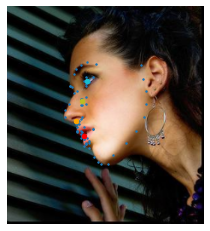
\includegraphics[width=5cm]{face_align_3.png}
    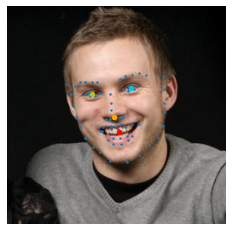
\includegraphics[width=5cm]{face_align_4.png}
    \caption[Visualisation of face landmarks, with certain landmarks highlighted.]{Visualisation of face landmarks, with certain landmarks highlighted. Images are from the  LS3D-W dataset\cite{bulat2017far_face_alignment}.}
    \label{fig:face_landmark_features}
\end{figure}


\subsection{Final Output}

Since we evaluate a video and not a single image, we expect to have multiple predictions for a single track. Some approach is needed to produce a final output of the algorithm. We designed the algorithm to finalize its decision once the track leaves the scene.

% mean, mode, median
Some statistical function is needed to process the multiple predictions into a single outcome. We think reasonable choices are mode for the gender prediction and median for the age prediction.

% 
If the given track has no associated prediction, we output its demographics as ``unknown'', as we have no prior knowledge about the class probabilities. Additionally, it might be reasonable to output ``unknown'' even when there is data present. For example, if there is an equal or almost equal number of predictions for the different gender classes.


\section{Algorithm Hyperparameters}

The presented algorithm has a number of hyperparameters that need to be configured. This section presents their overview and used values in table \ref{table:hyperparameters}. The values are presented mostly for illustrative purposes and as a potential starting point. Target scene, selected models and target goals must be considered when choosing the hyperparameters.

\begin{table}[htb]
    \centering
    
    \begin{tabularx}{\textwidth}{c|X|c}
        name & description & value \\
        \hline
        max\_age & Tracks missed more times are considered lost. & 7  \\
        max\_age\_active & Maximum track's age to be considered active. & 1 \\
        min\_hits & Minimum number of assigned detections to be considered confirmed. & 5 \\
        feature\_alpha & Weight for calculating new visual feature (higher means slower update). & 0.8 \\
        motion\_weight & Weight of the motion distance in contrast to visual feature distance (note that the motion distances are typically about an order larger). & 0.02 \\
        iou\_threshold & Minimal \gls{iou} to consider areas overlaping (when associating with \gls{iou}. & 0.5 \\
        measurement\_noise & Detected bounding box standard deviation. & 100 \\
        process\_noise\_var & Kalman filter process variance. & 10
    \end{tabularx}
    
    \caption{Selected algorithm hyperparameters.}
    \label{table:hyperparameters}
\end{table}

\section{Implementation}

The pipeline is implemented in Python 3.6. We use \textit{TensorRT} framework for optimized \gls{nn} inference on the Jetson platform. \textit{GStreamer} framework along with Jetson-specific NVIDIA plugins is used for efficient video stream processing. \cite{yukai_yang_2020_4294717_fastmot} was used as a basis for developing the pipeline, which proved especially helpful for efficient video processing and using the \textit{TensorRT} framework.

Used Python libraries are \textit{NumPy} for numerical computing and matrix operations, \textit{Pandas} for data manipulation, \textit{FilterPy} for Kalman filter implementation, \textit{py-motmetrics} for \gls{mot} metric calculations and \textit{OpenCV} for video and image processing.

\subsection{Inputs and Outputs}

The system should be usable with various input sources and produce output suitable for additional computer processing.

A standard protocol used in industrial and surveillance cameras is RTSP\cite{schulzrinne1998real_rtsp}. Handling input via this protocol allows the application to be easily connected to live streams from many types of cameras. The application also handles video input from the local filesystem to allow the processing of already recorded videos.

The application outputs location of all confirmed tracks for each frame along with their currently classified demographic information. The final demographic information is stored as a special event when a track leaves the scene. Output for the gender field is either male, female, or ``unknown''. For the age field, the output is either an age range or ``unknown''.

The application can optionally output the average frame rate and proportional time spend in various parts of the algorithms (time spent in detection, association, \dots{}). Additionally, the pipeline can be provided with \textit{ground truth} information for a given file and produce detailed statistics along with overall metrics.

Output can be either send periodically over the network or saved to the local filesystem. Data is saved in the JSON format, which is commonly used for data serialization.
\chapter{Experiments}\label{ch:experiments}

% fix url text overflow
\begin{sloppypar}
This chapter presents experiments and the evaluation of our algorithm. The goal of the experiments is to compare various models and approaches in terms of quality and performance. Supplementary materials and code are available at \url{https://github.com/davidmasek/Algorithms-for-video-analysis-of-customer-behavior-in-front-of-retail-store}.
\end{sloppypar}

All evaluations are run on the Jetson Xavier NX platform\cite{jetson}, with the 15W and 4 core power configuration. Jetpack version is 4.1.1, CUDA version is 10.2 and TensorRT version is 7.1.3.

\section{Tracker Evaluation}

The main part of our pipeline is the \gls{mot} tracker. We evaluate its performance on our collected dataset, which consists of 2600 annotated frames with 49 unique objects and 7108 objects in total. We split the dataset into train and test subsets, with respective sizes of 1309 and 1291 frames.

\begin{figure}[hbt!]
    \centering
    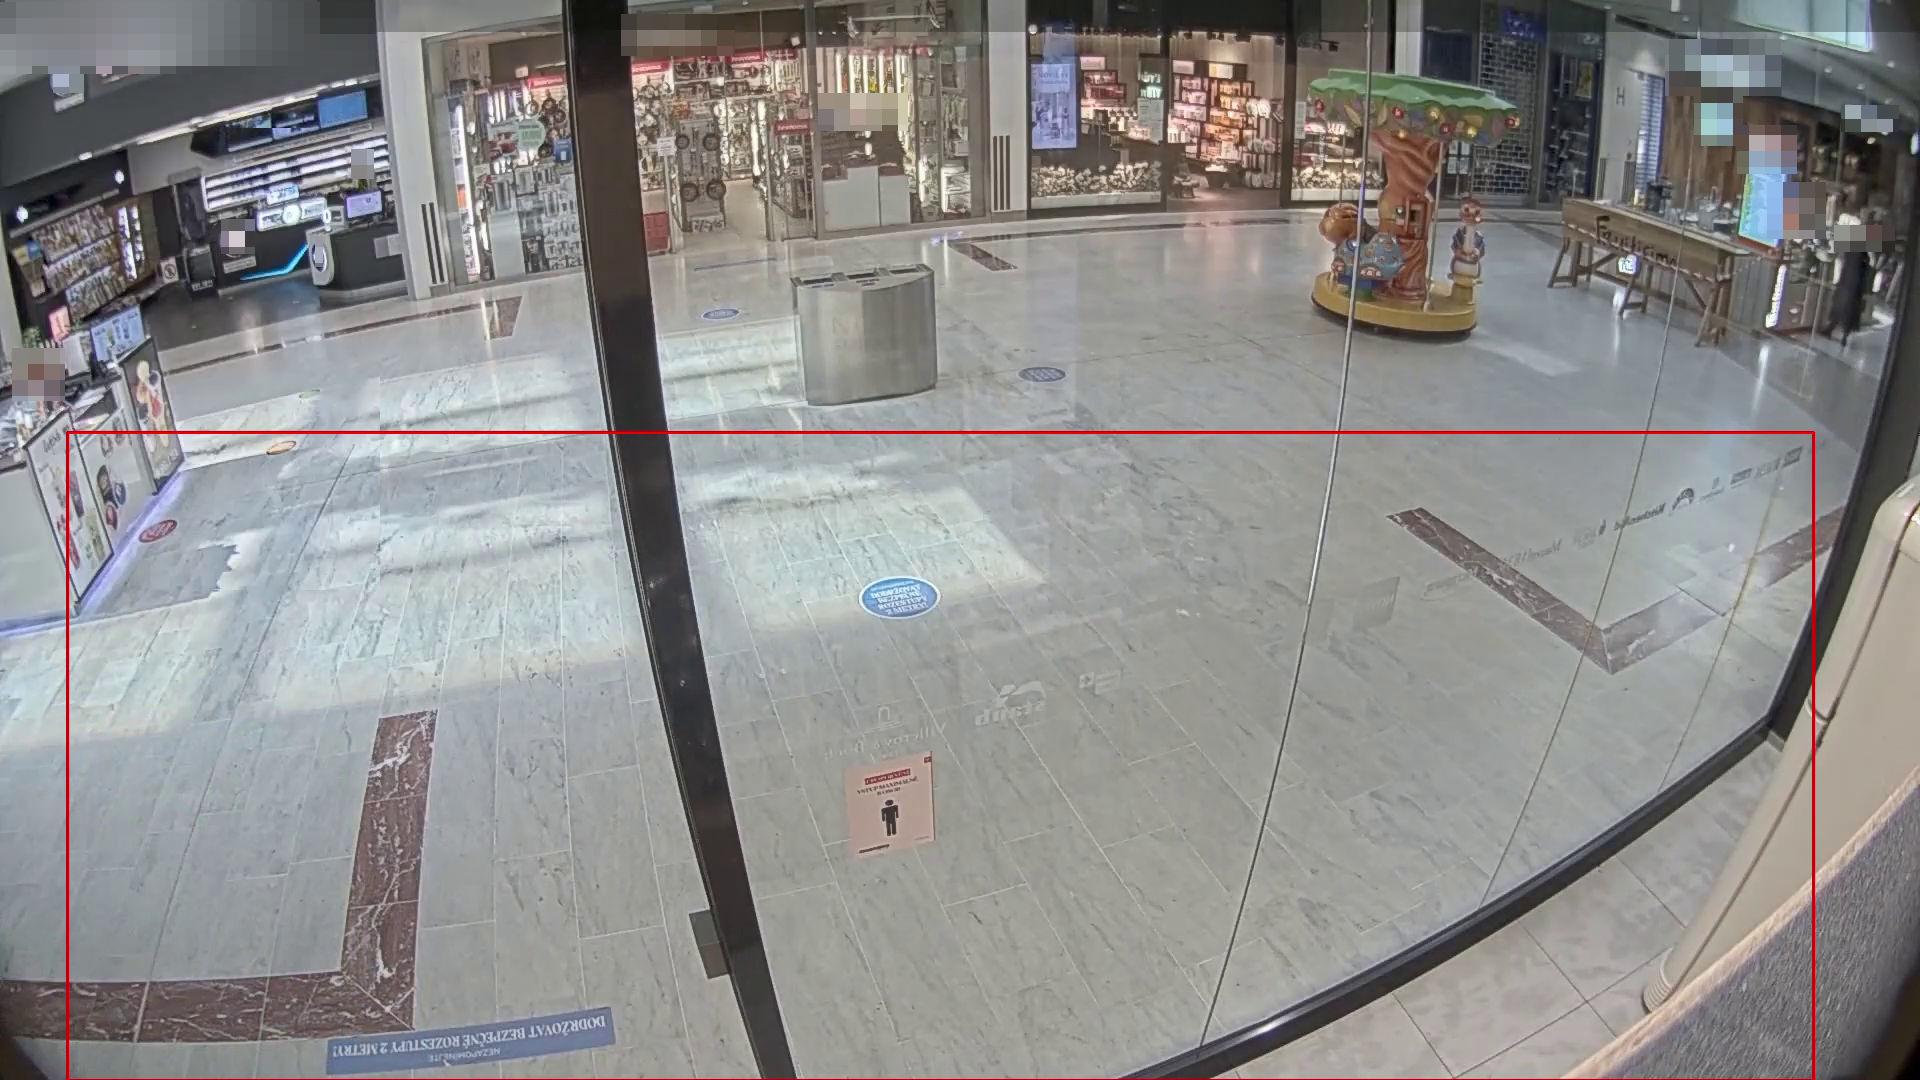
\includegraphics[width=8cm]{roi}
    \caption[A sample frame from the dataset with visualized \acrshort{roi}.]{A sample frame from the dataset with visualized \gls{roi}.}
    \label{fig:roi}
\end{figure}

We run the pipeline without the demographics extraction. We evaluate only tracks and annotations inside the \gls{roi}, a rectangle covering the relevant area in front of the shop. See figure \ref{fig:roi} for visualisation. Results are presented in table \ref{tab:tracker_results}. Final results are computed as an average of the evaluated sequences weighted by the number of frames. \textit{Switch ratio} is the ratio between the number of identity switches and the number of objects in total (scaled by 1000 for readability). We consider the minimal frame rate for real-time processing to be 10 \gls{fps}.

\textit{YOLOv4}\cite{bochkovskiy2020yolov4} is trained on the \textit{CrowdHuman}\cite{shao2018crowdhuman} dataset. \textit{PeopleNet}\cite{peoplenet} is trained on a proprietary NVIDIA dataset. The \textit{SSD}\cite{liu2016ssd} model is trained on the \textit{COCO}\cite{lin2014microsoft_coco} dataset and used with \textit{InceptionV2}\cite{ioffe2015batch_inception} as a feature extractor.

\begin{table}[hbt!]
    \centering
    \begin{tabular}{l|c|c|c|c}
        \hline
        Model & MOTA\,$\uparrow$ & MOTP\,$\uparrow$ & Switch Ratio\,$\downarrow$ & FPS\,$\uparrow$ \\
        \hline
        PeopleNet & 0.84 & 0.83 & \textbf{8.6} & 9.42 \\
        YOLOv4 & \textbf{0.91} & \textbf{0.93} & 8.7 & \textbf{13.0} \\
        SSD & 0.53 & 0.73 & 25 & 12.8
    \end{tabular}
    \caption{Tracker evaluation results with different detector models. The arrows indicate low or high optimal metric values.}
    \label{tab:tracker_results}
\end{table}

Based on the results, we selected the \textit{YOLOv4} model for use in the application. It has the best results in all categories except for the \textit{switch ratio}, where the results are very close to the best. Based on the metrics and visual evaluation of the algorithm's outputs, we consider its performance satisfactory.  We also consider the algorithm fast enough for real-time usage. 

Apart from our dataset, we also experimented on the MOT17\cite{MOT16} dataset, which is popular in literature. We have found the dataset to be too different from our target environment. The dataset contains videos taken from different angles and (often) with a moving camera. Our work assumes a stationary camera position at an elevated viewpoint, and so we have decided not to use the MOT17 dataset for evaluation. However, it remains an interesting source of data for testing the algorithm's robustness.

\section{Performance Optimization}

This section evaluates multiple architectures from a performance standpoint. In particular, we are interested in performance gain from using the TensorRT optimization framework.

We evaluate the \textit{SSRNet}\cite{yang2018ssr} and \textit{GoogLenet}\cite{szegedy2015going_googlenet} usable for age and gender classification. Further, we evaluate two \textit{OSNet}\cite{osnet} \gls{reid} architectures. As a baseline, we run the inference on CPU and GPU using \textit{ONNX Runtime}\cite{onnxruntime}, which is an open source machine learning framework. We then use the \textit{TensorRT} framework to optimize the model and run inference. The results are presented in table \ref{tab:cpu_gpu_trt}.

% ONNX runtime CPU, ONNX runtime GPU (CUDA), TensorRT (GPU - CUDA)
\begin{table}[hbt!]
    \centering
    \begin{tabular}{l|c|c|c}
        \hline
        Architecture & CPU & GPU & TensorRT \\
        \hline
        SSRNet (batch size 1) & 3.7 ms & 4.02 ms & 1.4 ms \\
        SSRNet (batch size 32) & 106 ms & 8.85 ms & 3.85 ms \\
        GoogLeNet & 144 ms & 12 ms & 3.17 ms \\
        \hline
        OSNet\_x0.25 & 361 ms & 41.8 ms & 12.3 ms \\
        OSNet\_ain\_x1.0 & 2.08 s & 156 ms & 53.8 ms
    \end{tabular}
    \caption{Inference time comparison.}
    \label{tab:cpu_gpu_trt}
\end{table}

We observe that using the \textit{TensorRT} optimized models increases performance about three times. To test that the optimization does not significantly decrease accuracy we evaluated the \textit{SSRNet} model on the \textit{MegaAge}\cite{huang2016unsupervised_megaage} dataset. The test \gls{mae} of the baseline version is  12.8, and the \gls{mae} of the optimized version is 14.4 (which is an error increase of 12.6\%).

Based on our experiments, we conclude that the \textit{TensorRT} framework can be used for significant performance gain while maintaining comparable results. However, it should be noted that the results may vary on different models or hardware.


\setsecnumdepth{part}
\chapter{Conclusion}
% automatically added to table of contents, so the lines below not required
% \addcontentsline{toc}{chapter}{Conclusion}
% \markboth{Conclusion}{Conclusion}

The goal of this thesis was to design and implement a  pipeline for tracking people in front of a retail store while also obtaining information about age and gender.

In the first two chapters, we presented necessary theoretical concepts and explored related works and existing approaches.

Next, we analyzed the requirements of the retail environment and potential solutions. To provide relevant evaluation, we collected a new dataset with cooperation from retail store owners. Collecting the dataset made us more aware of potential problems and helped in the algorithm design. Due to the current Covid19 epidemic, we were unable to include age and gender information in our dataset, which led us to focus on the tracking task and leave demographic feature extraction as a secondary objective.

Based on our analysis and research, we designed a \gls{mot} pipeline based on the \gls{deepsort} algorithm presented in \cite{Wojke2017_DeepSORT}. We modified the algorithm mainly in the association phase and extended it with the support for demographic information extraction. The tracking is based on associating new detections to existing tracks using the combination of two metrics. The first metric is \gls{iou} of Kalman filter predictions for tracks' locations and detections' bounding boxes. The second metric measures the visual similarity between detections and tracks.

Our pipeline is focused on performance and usability in the retail environment. We implemented the pipeline in Python using TensorRT framework for optimizations. The pipeline is optimized for the Jetson NX device, which has been chosen as a suitable device for production.

% Popsat, že jsme udělali nějaké experimenty, porovnali modely/parametry a napsat jak dopadlo nějaké vyhodnocení (evaluation)
In the last chapter, we presented experiments comparing various models and evaluated our application on the collected dataset. We concluded that the algorithm provides satisfactory results for use in production and can run in real time.

% future work and potential improvement (+ ImproLab plug?)
The most relevant opportunities for future improvement are demographic information extraction and overall robustness. Specifically, it would be beneficial to collect data from other locations and include the demographic information. We plan to continue working on the presented pipeline in cooperation with ImproLab laboratory at FIT CTU, with the goal of deploying the application in production.


\listoftodos


\bibliographystyle{meta/iso690}
\bibliography{ref}

\setsecnumdepth{all}
\appendix

% \chapter{Acronyms}

\newacronym{nn}{NN}{Neural Network}
\newacronym{mot}{MOT}{Multiple Object Tracking}
\newacronym{ai}{AI}{Artificial inteligence}
\newacronym{ml}{ML}{Machine learning}
\newacronym{mse}{MSE}{Mean Squared Error}
\newacronym{mae}{MAE}{Mean Average Error}
\newacronym{cnn}{CNN}{Convolutional Neural Network}
\newacronym{rgb}{RGB}{Red, Green, Blue}
\newacronym{iou}{IOU}{Intersection over Union}
\newacronym{reid}{ReID}{re-identification}
\newacronym{roi}{ROI}{Region of Interest}
\newacronym{sota}{SOTA}{state-of-the-art}
\newacronym{sort}{SORT}{Simple Online Realtime Tracking}
\newacronym{mota}{MOTA}{Multiple Object Tracking Accuracy}
\newacronym{motp}{MOTP}{Multiple Object Tracking Precision}
\newacronym{deepsort}{DeepSORT}{Simple Online and Realtime Tracking with a Deep Association Metric}
\newacronym{rtsp}{RTSP}{Real Time Streaming Protocol}
\newacronym{sdk}{SDK}{Software Development Kit}
\newacronym{fps}{FPS}{Frames Per Second}

\newacronym{Jetson}{Jetson}{Xavier Jetson NX}


\printglossaries

\chapter{Contents of enclosed CD}

%change appropriately

\begin{figure}
	\dirtree{%
		.1 readme.txt\DTcomment{the file with CD contents description}.
		.1 src\DTcomment{the directory of \LaTeX{} source codes of the thesis}.
		.1 thesis.pdf\DTcomment{the thesis text in PDF format}.
	}
\end{figure}

\end{document}
